% Copyright 2004 by Till Tantau <tantau@users.sourceforge.net>.
%
% In principle, this file can be redistributed and/or modified under
% the terms of the GNU Public License, version 2.
%
% However, this file is supposed to be a template to be modified
% for your own needs. For this reason, if you use this file as a
% template and not specifically distribute it as part of a another
% package/program, I grant the extra permission to freely copy and
% modify this file as you see fit and even to delete this copyright
% notice. 

\documentclass[aspectratio=169, handout, 10pt, hyperref=colorlinks]{beamer}

% There are many different themes available for Beamer. A comprehensive
% list with examples is given here:
% http://deic.uab.es/~iblanes/beamer_gallery/index_by_theme.html
% You can uncomment the themes below if you would like to use a different
% one:
%\usetheme{AnnArbor}
%\usetheme{Antibes}
%\usetheme{Bergen}
%\usetheme{Berkeley}
%\usetheme{Berlin}
\usetheme{Boadilla}
%\usetheme{boxes}
%\usetheme{CambridgeUS}
%\usetheme{Copenhagen}
%\usetheme{Darmstadt}
%\usetheme{default}
%\usetheme{Frankfurt}
%\usetheme{Goettingen}
%\usetheme{Hannover}
%\usetheme{Ilmenau}
%\usetheme{JuanLesPins}
%\usetheme{Luebeck}
% \usetheme{Madrid}
%\usetheme{Malmoe}
%\usetheme{Marburg}
%\usetheme{Montpellier}
%\usetheme{PaloAlto}
%\usetheme{Pittsburgh}
%\usetheme{Rochester}
%\usetheme{Singapore}
%\usetheme{Szeged}
%\usetheme{Warsaw}

\title{Data-Driven Analysis and Control using Informativity}
% A subtitle is optional and this may be deleted
\subtitle{EE593 Dual Degree Project - II}

% \author{F.~Author\inst{1} \and S.~Another\inst{2}}
\author[Param Rathour]{Rathour Param Jitendrakumar\\190070049}
% - Give the names in the same order as the appear in the paper.
% - Use the \inst{?} command only if the authors have different
%   affiliation.

\institute[IIT Bombay]{Department of Electrical Engineering\\
Indian Institute of Technology Bombay} % (optional, but mostly needed)
% {
%   \inst{1}%
%   Department of Computer Science\\
%   University of Somewhere
%   \and
%   \inst{2}%
%   Department of Theoretical Philosophy\\
%   University of Elsewhere}
% - Use the \inst command only if there are several affiliations.
% - Keep it simple, no one is interested in your street address.

\date{Autumn 2023-24}
% - Either use conference name or its abbreviation.
% - Not really informative to the audience, more for people (including
%   yourself) who are reading the slides online

\subject{Data-Driven Analysis and Control using Informativity}
% This is only inserted into the PDF information catalog. Can be left
% out. 

% If you have a file called "university-logo-filename.xxx", where xxx
% is a graphic format that can be processed by latex or pdflatex,
% resp., then you can add a logo as follows:

% \pgfdeclareimage[height=0.5cm]{university-logo}{university-logo-filename}
% \logo{\pgfuseimage{university-logo}}

% Delete this, if you do not want the table of contents to pop up at
% the beginning of each subsection:
% \AtBeginSubsection[]
% {
%   \begin{frame}<beamer>{Outline}
%     \tableofcontents[currentsection,currentsubsection]
%   \end{frame}
% }

\usepackage{braket}
% \usepackage{natbib}
\usepackage{epigraph}
\usepackage{fancyvrb}
\usepackage{amsmath,amssymb,amsfonts,mathtools,nccmath,bm}
\usepackage{algorithm}
\usepackage{algpseudocode}
\usepackage{graphicx}
\graphicspath{{./Images}}
\usepackage{textcomp}
\usepackage{xcolor}
\usepackage{float}
\usepackage{tikz}
\usepackage{pmat}
\usetikzlibrary{shapes,arrows.meta}
\tikzstyle{line} = [draw, -{Latex[length=1mm,width=2mm]}]
\tikzstyle{linedash} = [draw, dash dot]
% \hypersetup{colorlinks, linkcolor=magenta}
\usepackage{ragged2e}
% \usepackage{etoolbox}
% \apptocmd{\frame}{}{\justifying}{} % Allow optional arguments after frame.
\renewcommand{\raggedright}{\leftskip=0pt \rightskip=0pt plus 0cm}
\apptocmd{\frame}{}{\justifying}{}
% \addtobeamertemplate{}{}{\justifying}

\setbeamersize{text margin left=2em,text margin right=2em}

\newcommand*{\proofbreak}{\usebeamertemplate{proof end}\framebreak\usebeamertemplate{proof begin}}
\newcommand*{\enumbreak}{\usebeamertemplate{enumerate end}\framebreak\usebeamertemplate{enumerate begin}}

% \beamerdefaultoverlayspecification{<+->}
% \addtobeamertemplate{proof begin}{%
%     \setbeamercolor{block title}{fg=red!50!black,bg=red!25!white}%
%     \setbeamercolor{block body}{fg=black, bg=red!10!white}%
% }{}
% \newcommand{\lenitem}[2][.7\linewidth]{\parbox[t]{#1}{\strut #2\strut}}

\newtheorem{defn}{Definition}
\newtheorem{lem}{Lemma}
\newtheorem{prop}{Proposition}
\theoremstyle{example}
\newtheorem{postulate}{Postulate}
\newtheorem{assumption}{Assumption}
% \newtheorem{problem}{Problem}
% \newtheorem{note}{Note}

\renewcommand{\d}{\, \mathrm{d}}
\newcommand{\I}{\textbf{I}}
\newcommand{\V}{\textbf{V}}
% \newcommand{\F}{\ensuremath\mathbb{F}}
% \newcommand{\R}{\ensuremath\mathbb{R}}
% \newcommand{\C}{\ensuremath\mathbb{C}}
% \newcommand{\Q}{\ensuremath\mathbb{Q}}
% \newcommand{\Z}{\ensuremath\mathbb{Z}}
% \newcommand{\Zp}{\ensuremath\mathbb{Z}^+}
\newcommand{\lex}{\ensuremath>_{\text{lex}}}
\newcommand{\grlex}{\ensuremath>_{\text{grlex}}}
\newcommand{\grevlex}{\ensuremath>_{\text{grevlex}}}
\newcommand{\op}[1]{\operatorname{#1}}
\newcommand{\ditto}[1][.4pt]{\xrfill{#1}~\textquotedbl~\xrfill{#1}}
\newcommand{\suth}{\textsuperscript{th}}
\newcommand{\Grob}{Gr\"{o}bner }
\newcommand{\GrobB}{Gr\"{o}bner Bases}
\newcommand{\GrobBi}{Gr\"{o}bner Basis}
\renewcommand{\algorithmicrequire}{\textbf{Input:}}
\renewcommand{\algorithmicensure}{\textbf{Output:}}

% \usepackage{environ}
% \newcommand{\customframefont}[1]{
% \setbeamertemplate{itemize/enumerate body begin}{#1}
% \setbeamertemplate{itemize/enumerate subbody begin}{#1}
% }

% \NewEnviron{framefont}[1]{
% \customframefont{#1} % for itemize/enumerate
% {#1 % For the text outside itemize/enumerate
% \BODY
% }
% \customframefont{\normalsize}
% }
\newcommand{\XX}[1]{{\bf XX #1 XX}}
\newcommand{\bi}{\begin{itemize}}\newcommand{\ei}{\end{itemize}}
\newcommand{\be}{\begin{equation}}\newcommand{\ee}{\end{equation}}
\newcommand{\bee}{\begin{enumerate}}\newcommand{\eee}{\end{enumerate}}
\newcommand{\bea}{\begin{eqnarray}}\newcommand{\eea}{\end{eqnarray}}
\newcommand{\beas}{\begin{eqnarray*}}\newcommand{\eeas}{\end{eqnarray*}}

%



\newcommand{\bmf}{\mathbf{f}}
\newcommand{\bmu}{\mathbf{u}}
\newcommand{\bmx}{\mathbf{x}}
\newcommand{\bmv}{\mathbf{v}}
\newcommand{\bmw}{\mathbf{w}}
\newcommand{\bmy}{\mathbf{y}}
\newcommand{\bmd}{\mathbf{d}}
\newcommand{\bmr}{\mathbf{r}}
\newcommand{\bmz}{\mathbf{z}}
\newcommand{\bmphi}{\mathbf{\phi}}
\newcommand{\xm}{X_-}
\newcommand{\xp}{X_+}
\newcommand{\um}{U_-}
\newcommand{\ym}{Y_-}
\newcommand{\xmt}{X_-^\top}
\newcommand{\xpt}{X_+^\top}
\newcommand{\umt}{U_-^\top}
\newcommand{\ymt}{Y_-^\top}

%**********************************
\newcommand{\bpi}{\mathbf{\Pi}}
\newcommand{\schur}{\!\mid\!}
\newcommand{\mpi}{\bbm \Pi_{11}&\Pi_{12}\\\Pi_{21}&\Pi_{22}\ebm}
\newcommand{\gi}{^\dagger}
\renewcommand{\S}[1]{\mathbb{S}^{#1}}
\newcommand{\pip}{\Pi_{22}}
\newcommand{\pis}{\Pi\schur\Pi_{22}}
\newcommand{\zs}{\calZ_r(\Pi)}
\DeclareMathOperator{\In}{In}

\definecolor{marine}{rgb}{0.149,0.149,0.804}
\definecolor{fbrick}{rgb}{0.804,0.149,0.149}
\definecolor{apricot}{rgb}{0.98,0.81,0.69}
\definecolor{Blue}{cmyk}{1.,1.,0,0}
\definecolor{amber}{rgb}{1.0, 0.75, 0.0}
\definecolor{applegreen}{rgb}{0.55, 0.71, 0.0}
\definecolor{bananayellow}{rgb}{1.0, 0.88, 0.21}
\definecolor{bittersweet}{rgb}{1.0, 0.44, 0.37}
\definecolor{candyapplered}{rgb}{1.0, 0.03, 0.0}
\definecolor{carminered}{rgb}{1.0, 0.0, 0.22}
\definecolor{carrotorange}{rgb}{0.93, 0.57, 0.13}
\definecolor{goldenyellow}{rgb}{1.0, 0.87, 0.0}
\definecolor{greenpigment}{rgb}{0.0, 0.65, 0.31}
\definecolor{greenhtml}{rgb}{0.0, 0.5, 0.0}


\newcommand{\magenta}[1]{\textcolor{magenta}{#1}}
\newcommand{\fbrick}[1]{\textcolor{fbrick}{#1}}
\newcommand{\marine}[1]{\textcolor{marine}{#1}}
\newcommand{\green}[1]{\textcolor{greenpigment}{#1}}
\newcommand{\gray}[1]{\textcolor{gray}{#1}}

\newcommand{\ciz}{\hspace{5cm}{{\hrule}}\vspace*{4mm}}
\newcommand{\blue}{\textcolor{blue}}
\newcommand{\red}{\textcolor{red}}


\newcommand{\None}{
	\left[\begin{array}{c|c}
		I & \begin{array}{c}
			X_+\\Y_- 
		\end{array}
		\\\hline
		0 & \begin{array}{c}
			-X_-\\-U_- 
		\end{array}
	\end{array}\right]
	\!\!\!
	\bbm
	\Phi_{11} & \Phi_{12}\\
	\Phi_{21} & \Phi_{22}
	\ebm\!\!\!
	\left[\begin{array}{c|c}
		I & \begin{array}{c}
			X_+\\Y_- 
		\end{array}
		\\\hline
		0 & \begin{array}{c}
			-X_-\\-U_- 
		\end{array}
	\end{array}\right]^\top\!\!
}

\newcommand{\systwo}{
	\bbm
	I\\\hline\\[-3mm]
	\begin{matrix}
		A^\top & C^\top\!\\
		B^\top & D^\top\!
	\end{matrix}
	\ebm
}

\newcommand{\sysone}{
	\bbm
	I\\\hline\\[-3mm]
	\begin{matrix}
		A & B\\
		C & D
	\end{matrix}
	\ebm
}




%

%%%%%%%%%%%%%%%%%%%%%%%%%%%%%%%%%%%%%
%%                                 
%%  NEWCOMMANDS                    
%%                                 
%%  version 9  22/01/15           
%%                                 
%%%%%%%%%%%%%%%%%%%%%%%%%%%%%%%%%%%

%%%%%%%%%%%%%%%%%%%%%%%%%%%%%%%%%%%%
%
%
%%%%%%%%%%%%%%%%%%%%%%%%%%%%%%%%%%%



\DeclareMathOperator{\im}{im}
\DeclareMathOperator{\col}{col}
\DeclareMathOperator{\diag}{diag}
\DeclareMathOperator{\bdiag}{blockdiag}
\DeclareMathOperator{\spn}{span}
\DeclareMathOperator{\rank}{rank}
\DeclareMathOperator{\trace}{tr}
\DeclareMathOperator{\card}{card}
\DeclareMathOperator{\dist}{dist}
\DeclareMathOperator{\inte}{int}
\DeclareMathOperator{\clo}{cl}
\DeclareMathOperator{\rint}{rint}
\DeclareMathOperator{\conv}{conv}
\DeclareMathOperator{\cone}{cone}
\DeclareMathOperator{\dom}{dom}
\DeclareMathOperator{\graph}{graph}
\DeclareMathOperator{\dis}{dis}
\DeclareMathOperator{\Real}{Re}
\DeclareMathOperator{\Imag}{Im}




\let\leq\leqslant
\let\geq\geqslant
\let\emptyset\varnothing

%%%%%%%%%%%%%%%%%%%%%%%%%%%%%%%%%%%%%%%%%%%%%%%%
%     \calA
%%%%%%%%%%%%%%%%%%%%%%%%%%%%%%%%%%%%%%%%%%%%%%%%
\newcommand{\calA}{\ensuremath{\mathcal{A}}}
\newcommand{\calB}{\ensuremath{\mathcal{B}}}
\newcommand{\calC}{\ensuremath{\mathcal{C}}}
\newcommand{\calD}{\ensuremath{\mathcal{D}}}
\newcommand{\calE}{\ensuremath{\mathcal{E}}}
\newcommand{\calF}{\ensuremath{\mathcal{F}}}
\newcommand{\calG}{\ensuremath{\mathcal{G}}}
\newcommand{\calH}{\ensuremath{\mathcal{H}}}
\newcommand{\calI}{\ensuremath{\mathcal{I}}}
\newcommand{\calJ}{\ensuremath{\mathcal{J}}}
\newcommand{\calK}{\ensuremath{\mathcal{K}}}
\newcommand{\calL}{\ensuremath{\mathcal{L}}}
\newcommand{\calM}{\ensuremath{\mathcal{M}}}
\newcommand{\calN}{\ensuremath{\mathcal{N}}}
\newcommand{\calO}{\ensuremath{\mathcal{O}}}
\newcommand{\calP}{\ensuremath{\mathcal{P}}}
\newcommand{\calQ}{\ensuremath{\mathcal{Q}}}
\newcommand{\calR}{\ensuremath{\mathcal{R}}}
\newcommand{\calS}{\ensuremath{\mathcal{S}}}
\newcommand{\calT}{\ensuremath{\mathcal{T}}}
\newcommand{\calU}{\ensuremath{\mathcal{U}}}
\newcommand{\calV}{\ensuremath{\mathcal{V}}}
\newcommand{\calW}{\ensuremath{\mathcal{W}}}
\newcommand{\calX}{\ensuremath{\mathcal{X}}}
\newcommand{\calY}{\ensuremath{\mathcal{Y}}}
\newcommand{\calZ}{\ensuremath{\mathcal{Z}}}
%%%%%%%%%%%%%%%%%%%%%%%%%%%%%%%%%%%%%%%%%%%%%%%%
%     \sfA
%%%%%%%%%%%%%%%%%%%%%%%%%%%%%%%%%%%%%%%%%%%%%%%%
\newcommand{\sfA}{\ensuremath{\mathsf{A}}}
\newcommand{\sfB}{\ensuremath{\mathsf{B}}}
\newcommand{\sfC}{\ensuremath{\mathsf{C}}}
\newcommand{\sfD}{\ensuremath{\mathsf{D}}}
\newcommand{\sfE}{\ensuremath{\mathsf{E}}}
\newcommand{\sfF}{\ensuremath{\mathsf{F}}}
\newcommand{\sfG}{\ensuremath{\mathsf{G}}}
\newcommand{\sfH}{\ensuremath{\mathsf{H}}}
\newcommand{\sfI}{\ensuremath{\mathsf{I}}}
\newcommand{\sfJ}{\ensuremath{\mathsf{J}}}
\newcommand{\sfK}{\ensuremath{\mathsf{K}}}
\newcommand{\sfL}{\ensuremath{\mathsf{L}}}
\newcommand{\sfM}{\ensuremath{\mathsf{M}}}
\newcommand{\sfN}{\ensuremath{\mathsf{N}}}
\newcommand{\sfO}{\ensuremath{\mathsf{O}}}
\newcommand{\sfP}{\ensuremath{\mathsf{P}}}
\newcommand{\sfQ}{\ensuremath{\mathsf{Q}}}
\newcommand{\sfR}{\ensuremath{\mathsf{R}}}
\newcommand{\sfS}{\ensuremath{\mathsf{S}}}
\newcommand{\sfT}{\ensuremath{\mathsf{T}}}
\newcommand{\sfU}{\ensuremath{\mathsf{U}}}
\newcommand{\sfV}{\ensuremath{\mathsf{V}}}
\newcommand{\sfW}{\ensuremath{\mathsf{W}}}
\newcommand{\sfX}{\ensuremath{\mathsf{X}}}
\newcommand{\sfY}{\ensuremath{\mathsf{Y}}}
\newcommand{\sfZ}{\ensuremath{\mathsf{Z}}}
%%%%%%%%%%%%%%%%%%%%%%%%%%%%%%%%%%%%%%%%%%%%%%%%
%     \hata
%%%%%%%%%%%%%%%%%%%%%%%%%%%%%%%%%%%%%%%%%%%%%%%%
\newcommand{\hata}{\ensuremath{\hat{a}}}
\newcommand{\hatb}{\ensuremath{\hat{b}}}
\newcommand{\hatc}{\ensuremath{\hat{c}}}
\newcommand{\hatd}{\ensuremath{\hat{d}}}
\newcommand{\hate}{\ensuremath{\hat{e}}}
\newcommand{\hatf}{\ensuremath{\hat{f}}}
\newcommand{\hatg}{\ensuremath{\hat{g}}}
\newcommand{\hath}{\ensuremath{\hat{h}}}
\newcommand{\hati}{\ensuremath{\hat{i}}}
\newcommand{\hatj}{\ensuremath{\hat{j}}}
\newcommand{\hatk}{\ensuremath{\hat{k}}}
\newcommand{\hatl}{\ensuremath{\hat{l}}}
\newcommand{\hatm}{\ensuremath{\hat{m}}}
\newcommand{\hatn}{\ensuremath{\hat{n}}}
\newcommand{\hato}{\ensuremath{\hat{o}}}
\newcommand{\hatp}{\ensuremath{\hat{p}}}
\newcommand{\hatq}{\ensuremath{\hat{q}}}
\newcommand{\hatr}{\ensuremath{\hat{r}}}
\newcommand{\hats}{\ensuremath{\hat{s}}}
\newcommand{\hatt}{\ensuremath{\hat{t}}}
\newcommand{\hatu}{\ensuremath{\hat{u}}}
\newcommand{\hatv}{\ensuremath{\hat{v}}}
\newcommand{\hatw}{\ensuremath{\hat{w}}}
\newcommand{\hatx}{\ensuremath{\hat{x}}}
\newcommand{\haty}{\ensuremath{\hat{y}}}
\newcommand{\hatz}{\ensuremath{\hat{z}}}
%%%%%%%%%%%%%%%%%%%%%%%%%%%%%%%%%%%%%%%%%%%%%%%%
%     \hatA
%%%%%%%%%%%%%%%%%%%%%%%%%%%%%%%%%%%%%%%%%%%%%%%%
\newcommand{\hatA}{\ensuremath{\hat{A}}}
\newcommand{\hatB}{\ensuremath{\hat{B}}}
\newcommand{\hatC}{\ensuremath{\hat{C}}}
\newcommand{\hatD}{\ensuremath{\hat{D}}}
\newcommand{\hatE}{\ensuremath{\hat{E}}}
\newcommand{\hatF}{\ensuremath{\hat{F}}}
\newcommand{\hatG}{\ensuremath{\hat{G}}}
\newcommand{\hatH}{\ensuremath{\hat{H}}}
\newcommand{\hatI}{\ensuremath{\hat{I}}}
\newcommand{\hatJ}{\ensuremath{\hat{J}}}
\newcommand{\hatK}{\ensuremath{\hat{K}}}
\newcommand{\hatL}{\ensuremath{\hat{L}}}
\newcommand{\hatM}{\ensuremath{\hat{M}}}
\newcommand{\hatN}{\ensuremath{\hat{N}}}
\newcommand{\hatO}{\ensuremath{\hat{O}}}
\newcommand{\hatP}{\ensuremath{\hat{P}}}
\newcommand{\hatQ}{\ensuremath{\hat{Q}}}
\newcommand{\hatR}{\ensuremath{\hat{R}}}
\newcommand{\hatS}{\ensuremath{\hat{S}}}
\newcommand{\hatT}{\ensuremath{\hat{T}}}
\newcommand{\hatU}{\ensuremath{\hat{U}}}
\newcommand{\hatV}{\ensuremath{\hat{V}}}
\newcommand{\hatW}{\ensuremath{\hat{W}}}
\newcommand{\hatX}{\ensuremath{\hat{X}}}
\newcommand{\hatY}{\ensuremath{\hat{Y}}}
\newcommand{\hatZ}{\ensuremath{\hat{Z}}}
%%%%%%%%%%%%%%%%%%%%%%%%%%%%%%%%%%%%%%%%%%%%%%%%
%     \bara
%%%%%%%%%%%%%%%%%%%%%%%%%%%%%%%%%%%%%%%%%%%%%%%%
\newcommand{\bara}{\ensuremath{\bar{a}}}
\newcommand{\barb}{\ensuremath{\bar{b}}}
\newcommand{\barc}{\ensuremath{\bar{c}}}
\newcommand{\bard}{\ensuremath{\bar{d}}}
\newcommand{\bare}{\ensuremath{\bar{e}}}
\newcommand{\barf}{\ensuremath{\bar{f}}}
\newcommand{\barg}{\ensuremath{\bar{g}}}
\newcommand{\barh}{\ensuremath{\bar{h}}}
\newcommand{\bari}{\ensuremath{\bar{i}}}
\newcommand{\barj}{\ensuremath{\bar{j}}}
\newcommand{\bark}{\ensuremath{\bar{k}}}
\newcommand{\barl}{\ensuremath{\bar{l}}}
\newcommand{\barm}{\ensuremath{\bar{m}}}
\newcommand{\barn}{\ensuremath{\bar{n}}}
\newcommand{\baro}{\ensuremath{\bar{o}}}
\newcommand{\barp}{\ensuremath{\bar{p}}}
\newcommand{\barq}{\ensuremath{\bar{q}}}
\newcommand{\barr}{\ensuremath{\bar{r}}}
\newcommand{\bars}{\ensuremath{\bar{s}}}
\newcommand{\bart}{\ensuremath{\bar{t}}}
\newcommand{\baru}{\ensuremath{\bar{u}}}
\newcommand{\barv}{\ensuremath{\bar{v}}}
\newcommand{\barw}{\ensuremath{\bar{w}}}
\newcommand{\barx}{\ensuremath{\bar{x}}}
\newcommand{\bary}{\ensuremath{\bar{y}}}
\newcommand{\barz}{\ensuremath{\bar{z}}}
%%%%%%%%%%%%%%%%%%%%%%%%%%%%%%%%%%%%%%%%%%%%%%%%
%     \barA
%%%%%%%%%%%%%%%%%%%%%%%%%%%%%%%%%%%%%%%%%%%%%%%%
\newcommand{\barA}{\ensuremath{\bar{A}}}
\newcommand{\barB}{\ensuremath{\bar{B}}}
\newcommand{\barC}{\ensuremath{\bar{C}}}
\newcommand{\barD}{\ensuremath{\bar{D}}}
\newcommand{\barE}{\ensuremath{\bar{E}}}
\newcommand{\barF}{\ensuremath{\bar{F}}}
\newcommand{\barG}{\ensuremath{\bar{G}}}
\newcommand{\barH}{\ensuremath{\bar{H}}}
\newcommand{\barI}{\ensuremath{\bar{I}}}
\newcommand{\barJ}{\ensuremath{\bar{J}}}
\newcommand{\barK}{\ensuremath{\bar{K}}}
\newcommand{\barL}{\ensuremath{\bar{L}}}
\newcommand{\barM}{\ensuremath{\bar{M}}}
\newcommand{\barN}{\ensuremath{\bar{N}}}
\newcommand{\barO}{\ensuremath{\bar{O}}}
\newcommand{\barP}{\ensuremath{\bar{P}}}
\newcommand{\barQ}{\ensuremath{\bar{Q}}}
\newcommand{\barR}{\ensuremath{\bar{R}}}
\newcommand{\barS}{\ensuremath{\bar{S}}}
\newcommand{\barT}{\ensuremath{\bar{T}}}
\newcommand{\barU}{\ensuremath{\bar{U}}}
\newcommand{\barV}{\ensuremath{\bar{V}}}
\newcommand{\barW}{\ensuremath{\bar{W}}}
\newcommand{\barX}{\ensuremath{\bar{X}}}
\newcommand{\barY}{\ensuremath{\bar{Y}}}
\newcommand{\barZ}{\ensuremath{\bar{Z}}}
%%%%%%%%%%%%%%%%%%%%%%%%%%%%%%%%%%%%%%%%%%%%%%%%
%     \bbA
%%%%%%%%%%%%%%%%%%%%%%%%%%%%%%%%%%%%%%%%%%%%%%%%
\newcommand{\bbA}{\ensuremath{\mathbb{A}}}
\newcommand{\bbB}{\ensuremath{\mathbb{B}}}
\newcommand{\bbC}{\ensuremath{\mathbb{C}}}
\newcommand{\bbD}{\ensuremath{\mathbb{D}}}
\newcommand{\bbE}{\ensuremath{\mathbb{E}}}
\newcommand{\bbF}{\ensuremath{\mathbb{F}}}
\newcommand{\bbG}{\ensuremath{\mathbb{G}}}
\newcommand{\bbH}{\ensuremath{\mathbb{H}}}
\newcommand{\bbI}{\ensuremath{\mathbb{I}}}
\newcommand{\bbJ}{\ensuremath{\mathbb{J}}}
\newcommand{\bbK}{\ensuremath{\mathbb{K}}}
\newcommand{\bbL}{\ensuremath{\mathbb{L}}}
\newcommand{\bbM}{\ensuremath{\mathbb{M}}}
\newcommand{\bbN}{\ensuremath{\mathbb{N}}}
\newcommand{\bbO}{\ensuremath{\mathbb{O}}}
\newcommand{\bbP}{\ensuremath{\mathbb{P}}}
\newcommand{\bbQ}{\ensuremath{\mathbb{Q}}}
\newcommand{\bbR}{\ensuremath{\mathbb{R}}}
\newcommand{\bbS}{\ensuremath{\mathbb{S}}}
\newcommand{\bbT}{\ensuremath{\mathbb{T}}}
\newcommand{\bbU}{\ensuremath{\mathbb{U}}}
\newcommand{\bbV}{\ensuremath{\mathbb{V}}}
\newcommand{\bbW}{\ensuremath{\mathbb{W}}}
\newcommand{\bbX}{\ensuremath{\mathbb{X}}}
\newcommand{\bbY}{\ensuremath{\mathbb{Y}}}
\newcommand{\bbZ}{\ensuremath{\mathbb{Z}}}

%%%%%%%%%%%%%%%%%%%%%%%%%%%%%%%%%%%%%%%%%%%%%%%%
%     \tta
%%%%%%%%%%%%%%%%%%%%%%%%%%%%%%%%%%%%%%%%%%%%%%%%
\newcommand{\tta}{{\tt a}}
\newcommand{\ttb}{{\tt b}}
\newcommand{\ttc}{{\tt c}}
\newcommand{\ttd}{{\tt d}}
\newcommand{\tte}{{\tt e}}
\newcommand{\ttf}{{\tt f}}
\newcommand{\ttg}{{\tt g}}
\newcommand{\tth}{{\tt h}}
\newcommand{\tti}{{\tt i}}
\newcommand{\ttj}{{\tt j}}
\newcommand{\ttk}{{\tt k}}
\newcommand{\ttl}{{\tt l}}
\newcommand{\ttm}{{\tt m}}
\newcommand{\ttn}{{\tt n}}
\newcommand{\tto}{{\tt o}}
\newcommand{\ttp}{{\tt p}}
\newcommand{\ttq}{{\tt q}}
\newcommand{\ttr}{{\tt r}}
\newcommand{\tts}{{\tt s}}
\newcommand{\ttt}{{\tt t}}
\newcommand{\ttu}{{\tt u}}
\newcommand{\ttv}{{\tt v}}
\newcommand{\ttw}{{\tt w}}
\newcommand{\ttx}{{\tt x}}
\newcommand{\tty}{{\tt y}}
\newcommand{\ttz}{{\tt z}}


%%%%%%%%%%%%%%%%%%%%%%%%%%%%%%%%%%%%%%%%%%%%%
% ENVIRONMENTS
%%%%%%%%%%%%%%%%%%%%%%%%%%%%%%%%%%%%%%%%%%%%%
\newcommand{\bmat}{\begin{matrix}}
\newcommand{\emat}{\end{matrix}}
\newcommand{\bbm}{\begin{bmatrix}}
\newcommand{\ebm}{\end{bmatrix}}
\newcommand{\bbma}{\begin{bmatrix*}[r]}
\newcommand{\ebma}{\end{bmatrix*}}
\newcommand{\bpm}{\begin{pmatrix}}
\newcommand{\epm}{\end{pmatrix}}
\newcommand{\bvm}{\begin{vmatrix}}
\newcommand{\evm}{\end{vmatrix}}
\newcommand{\bse}{\begin{subequations}}
\newcommand{\ese}{\end{subequations}}
\newcommand{\beq}{\begin{equation}}
\newcommand{\eeq}{\end{equation}}
\newcommand{\ben}{\renewcommand{\labelenumi}{\arabic{enumi}.}
\renewcommand{\theenumi}{\arabic{enumi}}\begin{enumerate}}

\newcommand{\een}{\end{enumerate}}

\newcommand{\beni}{\renewcommand{\labelenumi}{\roman{enumi}.}
\renewcommand{\theenumi}{\roman{enumi}}\begin{enumerate}}

\newcommand{\eeni}{\end{enumerate}}

\newcommand{\bena}{\renewcommand{\labelenumi}{\alph{enumi}.}
\renewcommand{\theenumi}{\alph{enumi}}\begin{enumerate}}

\newcommand{\eena}{\end{enumerate}}

\newcommand{\bit}{\begin{itemize}}
\newcommand{\eit}{\end{itemize}}
\newcommand{\bthe}{\begin{theorem}}
\newcommand{\ethe}{\end{theorem}}
\newcommand{\blem}{\begin{lemma}}
\newcommand{\elem}{\end{lemma}}
\newcommand{\bprop}{\begin{proposition}}
\newcommand{\eprop}{\end{proposition}}
\newcommand{\bex}{\begin{example}}
\newcommand{\eex}{\end{example}}
\newcommand{\bas}{\begin{assumption}}
\newcommand{\eas}{\end{assumption}}
\newcommand{\bre}{\begin{remark}}
\newcommand{\ere}{\end{remark}}
\newcommand{\bcor}{\begin{corollary}}
\newcommand{\ecor}{\end{corollary}}
\newcommand{\bdfn}{\begin{definition}}
\newcommand{\edfn}{\end{definition}}
\newcommand{\bcon}{\begin{conjecture}}
\newcommand{\econ}{\end{conjecture}}


%%%%%%%%%%%%%%%%%%%%%%%%%%%%%%%%%%%%%%%%%%%%
%  NEW OPERATORS
%%%%%%%%%%%%%%%%%%%%%%%%%%%%%%%%%%%%%%%%%%%%

%%%%%%%%%%%%%%%%%%%%%%%%%%%%%%%%%%%%%%%%%%%%
%  SHORTHAND MATH
%%%%%%%%%%%%%%%%%%%%%%%%%%%%%%%%%%%%%%%%%%%%
\newcommand{\ones}{\ensuremath{1\!\!1}}
\newcommand{\eps}{\ensuremath{\varepsilon}}
\newcommand{\half}{\ensuremath{\frac{1}{2}}}
\newcommand{\inv}{\ensuremath{^{-1}}}
\newcommand{\pset}[1]{\ensuremath{\{#1\}}}
\newcommand{\nset}[1]{\ensuremath{\{1,2,\ldots,#1\}}}
\newcommand{\zset}{\ensuremath{\pset{0}}}
\newcommand{\lexleq}{\ensuremath{\preccurlyeq}}
\newcommand{\lexgeq}{\ensuremath{\succcurlyeq}}
% \newcommand{\set}[2]{\ensuremath{\{#1\mid #2\}}}
\newcommand{\res}[2]{\ensuremath{#1|_{#2}}}
\newcommand{\abs}[1]{\ensuremath{| #1 |}}
\newcommand{\norm}[1]{\ensuremath{\| #1 \|}}
\newcommand{\inn}[2]{\ensuremath{\langle #1 , #2 \rangle}}
\newcommand{\polar}[1]{\ensuremath{{#1}^\circ}}
\newcommand{\dual}[1]{\ensuremath{{#1}^*}}
\newcommand{\barrier}[1]{\ensuremath{{#1}^{\mathrm{b}}}}
\newcommand{\rec}[1]{\ensuremath{{#1}^{\infty}}}

%%%%%%%%%%%%%%%%%%%%%%%%%%%%%%%%%%%%%%%%%%%%
%  SETS
%%%%%%%%%%%%%%%%%%%%%%%%%%%%%%%%%%%%%%%%%%%%
\newcommand{\F}{\ensuremath\mathbb{F}}
\newcommand{\R}{\ensuremath\mathbb{R}}
\newcommand{\C}{\ensuremath\mathbb{C}}
\newcommand{\Q}{\ensuremath\mathbb{Q}}
\newcommand{\N}{\ensuremath{\mathbb N}}
\newcommand{\Z}{\ensuremath\mathbb{Z}}
\newcommand{\Zp}{\ensuremath\mathbb{Z}^+}
\newcommand{\Lone}{\ensuremath{L_1}}
\newcommand{\Loneloc}{\ensuremath{L_{1,\mathrm{loc}}}}
\newcommand{\Ltwo}{\ensuremath{L_2}}
\newcommand{\Ltwoloc}{\ensuremath{L_{2,\mathrm{loc}}}}
\newcommand{\Linf}{\ensuremath{L_\infty}}
\newcommand{\Linfloc}{\ensuremath{L_{\infty,\mathrm{loc}}}}
\newcommand{\Cinf}{\ensuremath{C^\infty}}
\newcommand{\Absc}{\ensuremath{\mathrm{AC}}}

%%%%%%%%%%%%%%%%%%%%%%%%%%%%%%%%%%%%%%%%%%%%
%  GEOMETRIC CONTROL
%%%%%%%%%%%%%%%%%%%%%%%%%%%%%%%%%%%%%%%%%%%%
\newcommand{\br}[2]{\ensuremath{\langle #1 \mid \im #2 \rangle}}
\newcommand{\brd}[2]{\ensuremath{\langle \ker #1 \mid #2 \rangle}}
\newcommand{\brn}[2]{\ensuremath{\langle #1 \mid #2 \rangle}}
\newcommand{\calVs}{\ensuremath{\calV^*}}
\newcommand{\calRs}{\ensuremath{\calR^*}}
\newcommand{\calTs}{\ensuremath{\calT^*}}

%%%%%%%%%%%%%%%%%%%%%%%%%%%%%%%%%%%%%%%%%%%%
%  SYSTEMS
%%%%%%%%%%%%%%%%%%%%%%%%%%%%%%%%%%%%%%%%%%%%
\newcommand{\abcd}{\ensuremath{(A,B,C,D)}}
\newcommand{\abcdef}{\ensuremath{(A,B,C,D,E,F)}}

%%%%%%%%%%%%%%%%%%%%%%%%%%%%%%%%%%%%%%%%%%%%
%  MISC
%%%%%%%%%%%%%%%%%%%%%%%%%%%%%%%%%%%%%%%%%%%%
\newcommand{\BP}{\noindent{\bf Proof. }}
\newcommand{\EP}{\hspace*{\fill} $\blacksquare$\bigskip\noindent}
\newcommand{\qand}{\quad\text{ and }\quad}








\newcommand{\ba}{\mathbf{a}}
\newcommand{\bb}{\mathbf{b}}
\newcommand{\bc}{\mathbf{c}}
\newcommand{\bd}{\mathbf{d}}
\renewcommand{\bf}{\mathbf{f}}
\newcommand{\bg}{\mathbf{g}}
\renewcommand{\bm}{\mathbf{m}}
\newcommand{\bs}{\mathbf{s}}
\newcommand{\bhs}{\mathbf{\hat{s}}}
\newcommand{\btz}{\mathbf{\tilde{z}}}
\newcommand{\bu}{\mathbf{u}}
\newcommand{\bv}{\mathbf{v}}
\newcommand{\bw}{\mathbf{w}}
\newcommand{\bwhat}{\mathbf{\hat{w}}}
\newcommand{\bx}{\mathbf{x}}
\newcommand{\bxhat}{\mathbf{\hat{x}}}
\newcommand{\bxtilde}{\mathbf{\tilde{x}}}
\newcommand{\by}{\mathbf{y}}
\newcommand{\bz}{\mathbf{z}}
\newcommand{\bA}{\mathbf{A}}
\newcommand{\bB}{\mathbf{B}}
\newcommand{\bC}{\mathbf{C}}
\newcommand{\bD}{\mathbf{D}}
\newcommand{\bF}{\mathbf{F}}
\newcommand{\bG}{\mathbf{G}}
\newcommand{\bH}{\mathbf{H}}
\newcommand{\bI}{\mathbf{I}}
\newcommand{\bJ}{\mathbf{J}}
\newcommand{\bL}{\mathbf{L}}
\newcommand{\bK}{\mathbf{K}}
\newcommand{\bN}{\mathbf{N}}
\newcommand{\bPtilde}{\bPhitilde}
\newcommand{\bPhat}{\mathbf{\hat{P}}}
\newcommand{\bQ}{\mathbf{Q}}
\newcommand{\bR}{\mathbf{R}}
\newcommand{\bS}{\mathbf{S}}
\newcommand{\bP}{\mathbf{P}}
\newcommand{\bT}{\mathbf{T}}
\newcommand{\bU}{\mathbf{U}}
\newcommand{\bV}{\mathbf{V}}
\newcommand{\bW}{\mathbf{W}}
\newcommand{\bX}{\mathbf{X}}
\newcommand{\bY}{\mathbf{Y}}
\newcommand{\bZ}{\mathbf{Z}}
\newcommand{\balpha}{\boldsymbol{\alpha}}
\newcommand{\bAtilde}{\mathbf{\tilde{A}}}
\newcommand{\bBtilde}{\mathbf{\tilde{B}}}
\newcommand{\bCtilde}{\mathbf{\tilde{C}}}
\newcommand{\bDtilde}{\mathbf{\tilde{D}}}
\newcommand{\bUtilde}{\mathbf{\tilde{U}}}
\newcommand{\bVtilde}{\mathbf{\tilde{V}}}
\newcommand{\bSigmatilde}{\boldsymbol{\tilde{\Sigma}}}
\newcommand{\bXtilde}{\mathbf{\tilde{X}}}
\newcommand{\bAhat}{\mathbf{\hat{A}}}
\newcommand{\bBhat}{\mathbf{\hat{B}}}
\newcommand{\bChat}{\mathbf{\hat{C}}}
\newcommand{\bDhat}{\mathbf{\hat{D}}}
\newcommand{\bWhat}{\mathbf{\hat{W}}}
\newcommand{\bchi}{\boldsymbol{\chi}}
\newcommand{\bxi}{\boldsymbol{\xi}}
\newcommand{\bXi}{\boldsymbol{\Xi}}
\newcommand{\bfeta}{\boldsymbol{\eta}}
\newcommand{\bmuu}{\boldsymbol{\mu}}
\newcommand{\bpsi}{\boldsymbol{\psi}}
\newcommand{\bPsi}{\boldsymbol{\Psi}}
\newcommand{\bphi}{\boldsymbol{\phi}}
\newcommand{\bPhi}{\boldsymbol{\Phi}}
\newcommand{\bGamma}{\boldsymbol{\Gamma}}
\newcommand{\bSigma}{\boldsymbol{\Sigma}}
\newcommand{\bTheta}{\boldsymbol{\Theta}}
\newcommand{\bUpsilon}{\boldsymbol{\Upsilon}}
\newcommand{\blambda}{\boldsymbol{\lambda}}
\newcommand{\bLambda}{\boldsymbol{\Lambda}}
\newcommand{\bOmega}{\boldsymbol{\Omega}}
\newcommand{\bPsitilde}{\boldsymbol{\tilde{\Psi}}}
\newcommand{\bPhitilde}{\boldsymbol{\tilde{\Phi}}}
\newcommand{\bPhihat}{\boldsymbol{\hat{\Phi}}}
\DeclareMathOperator*{\argmax}{arg\rm{}max}
\DeclareMathOperator*{\argmin}{arg\rm{}min}
\newcommand{\vect}[1]{\accentset{\rightharpoonup}{#1}}

\newcommand{\flow}{\ensuremath{\mathbf{F}}}
\newcommand{\koop}{\ensuremath{\mathcal{K}}}
\newcommand{\pf}{\ensuremath{\mathcal{P}}}
\newcommand{\gen}{\ensuremath{\mathcal{L}}}

\DeclareMathOperator{\lspan}{span}
\DeclarePairedDelimiter{\avg}{\langle}{\rangle}
\DeclarePairedDelimiter{\normlv}{\lVert}{\rVert}
\DeclarePairedDelimiter{\abslv}{\lvert}{\rvert}
\newcommand{\corr}[1][g]{C_{#1}}
% Let's get started
\begin{document}

\begin{frame}
  \titlepage
  \begin{center}
    Guide: Prof. Debasattam Pal
  \end{center}
%   \epigraph{When you go to sleep make sure there is someone to wake you up.}{Prof. Mythili Vutukuru}
\end{frame}

\begin{frame}[allowframebreaks]{Outline}
  \tableofcontents
  % You might wish to add the option [pausesections]
\end{frame}

% Section and subsections will appear in the presentation overview
% and table of contents.
\section{Introduction}
\subsection{Challenges in Modern Dynamical Systems}
\begin{frame}{Challenges in Modern Dynamical Systems}{Introduction}
  \begin{description}
  \item[Nonlinearity]
  Linear systems are simple and desirable. But nonlinear aren't. 

  Can perform local linearizations around fixed points, periodic orbits, etc. but predicting global phenomena is tough
  \item[Noise in the modelled data]
  Noise changes the entire dynamical system and in most cases it will result in losing linearity of the system which leads to the above mentioned problems
  \item[Unknown dynamics] Basic lack of physical laws governing systems in fields such as neuroscience, epidemiology, and ecology which tackle complex realistic systems.

  Even for known dynamics are like in turbulence, and protein folding, with higher dimensions uncovering dominant behviour is difficult.
  \end{description}
\end{frame}
\begin{frame}{Possible Solutions}{Introduction}
  \begin{description}
    \item[Informativity approach] With this framework, we convert the control problem in our hand to a Linear Matrix Inequality (LMI). For some control problems, specific noise models can also be accomodated in its analysis making it a robust solution.
    \item[Operator-theoretic representations] Using Koopman operator, we can represent nonlinear dynamical systems in terms of infinite-dimensional linear operators
    \item[Data-driven regression and machine learning] is becoming a critical tool to discover discover dynamical systems from data and it forms the basis of DMD, SINDy.% and other data-driven Koopman methods discussed later.
  \end{description}
\end{frame}
\begin{frame}{Dynamic Mode Decomposition (DMD)}
    \begin{figure}
        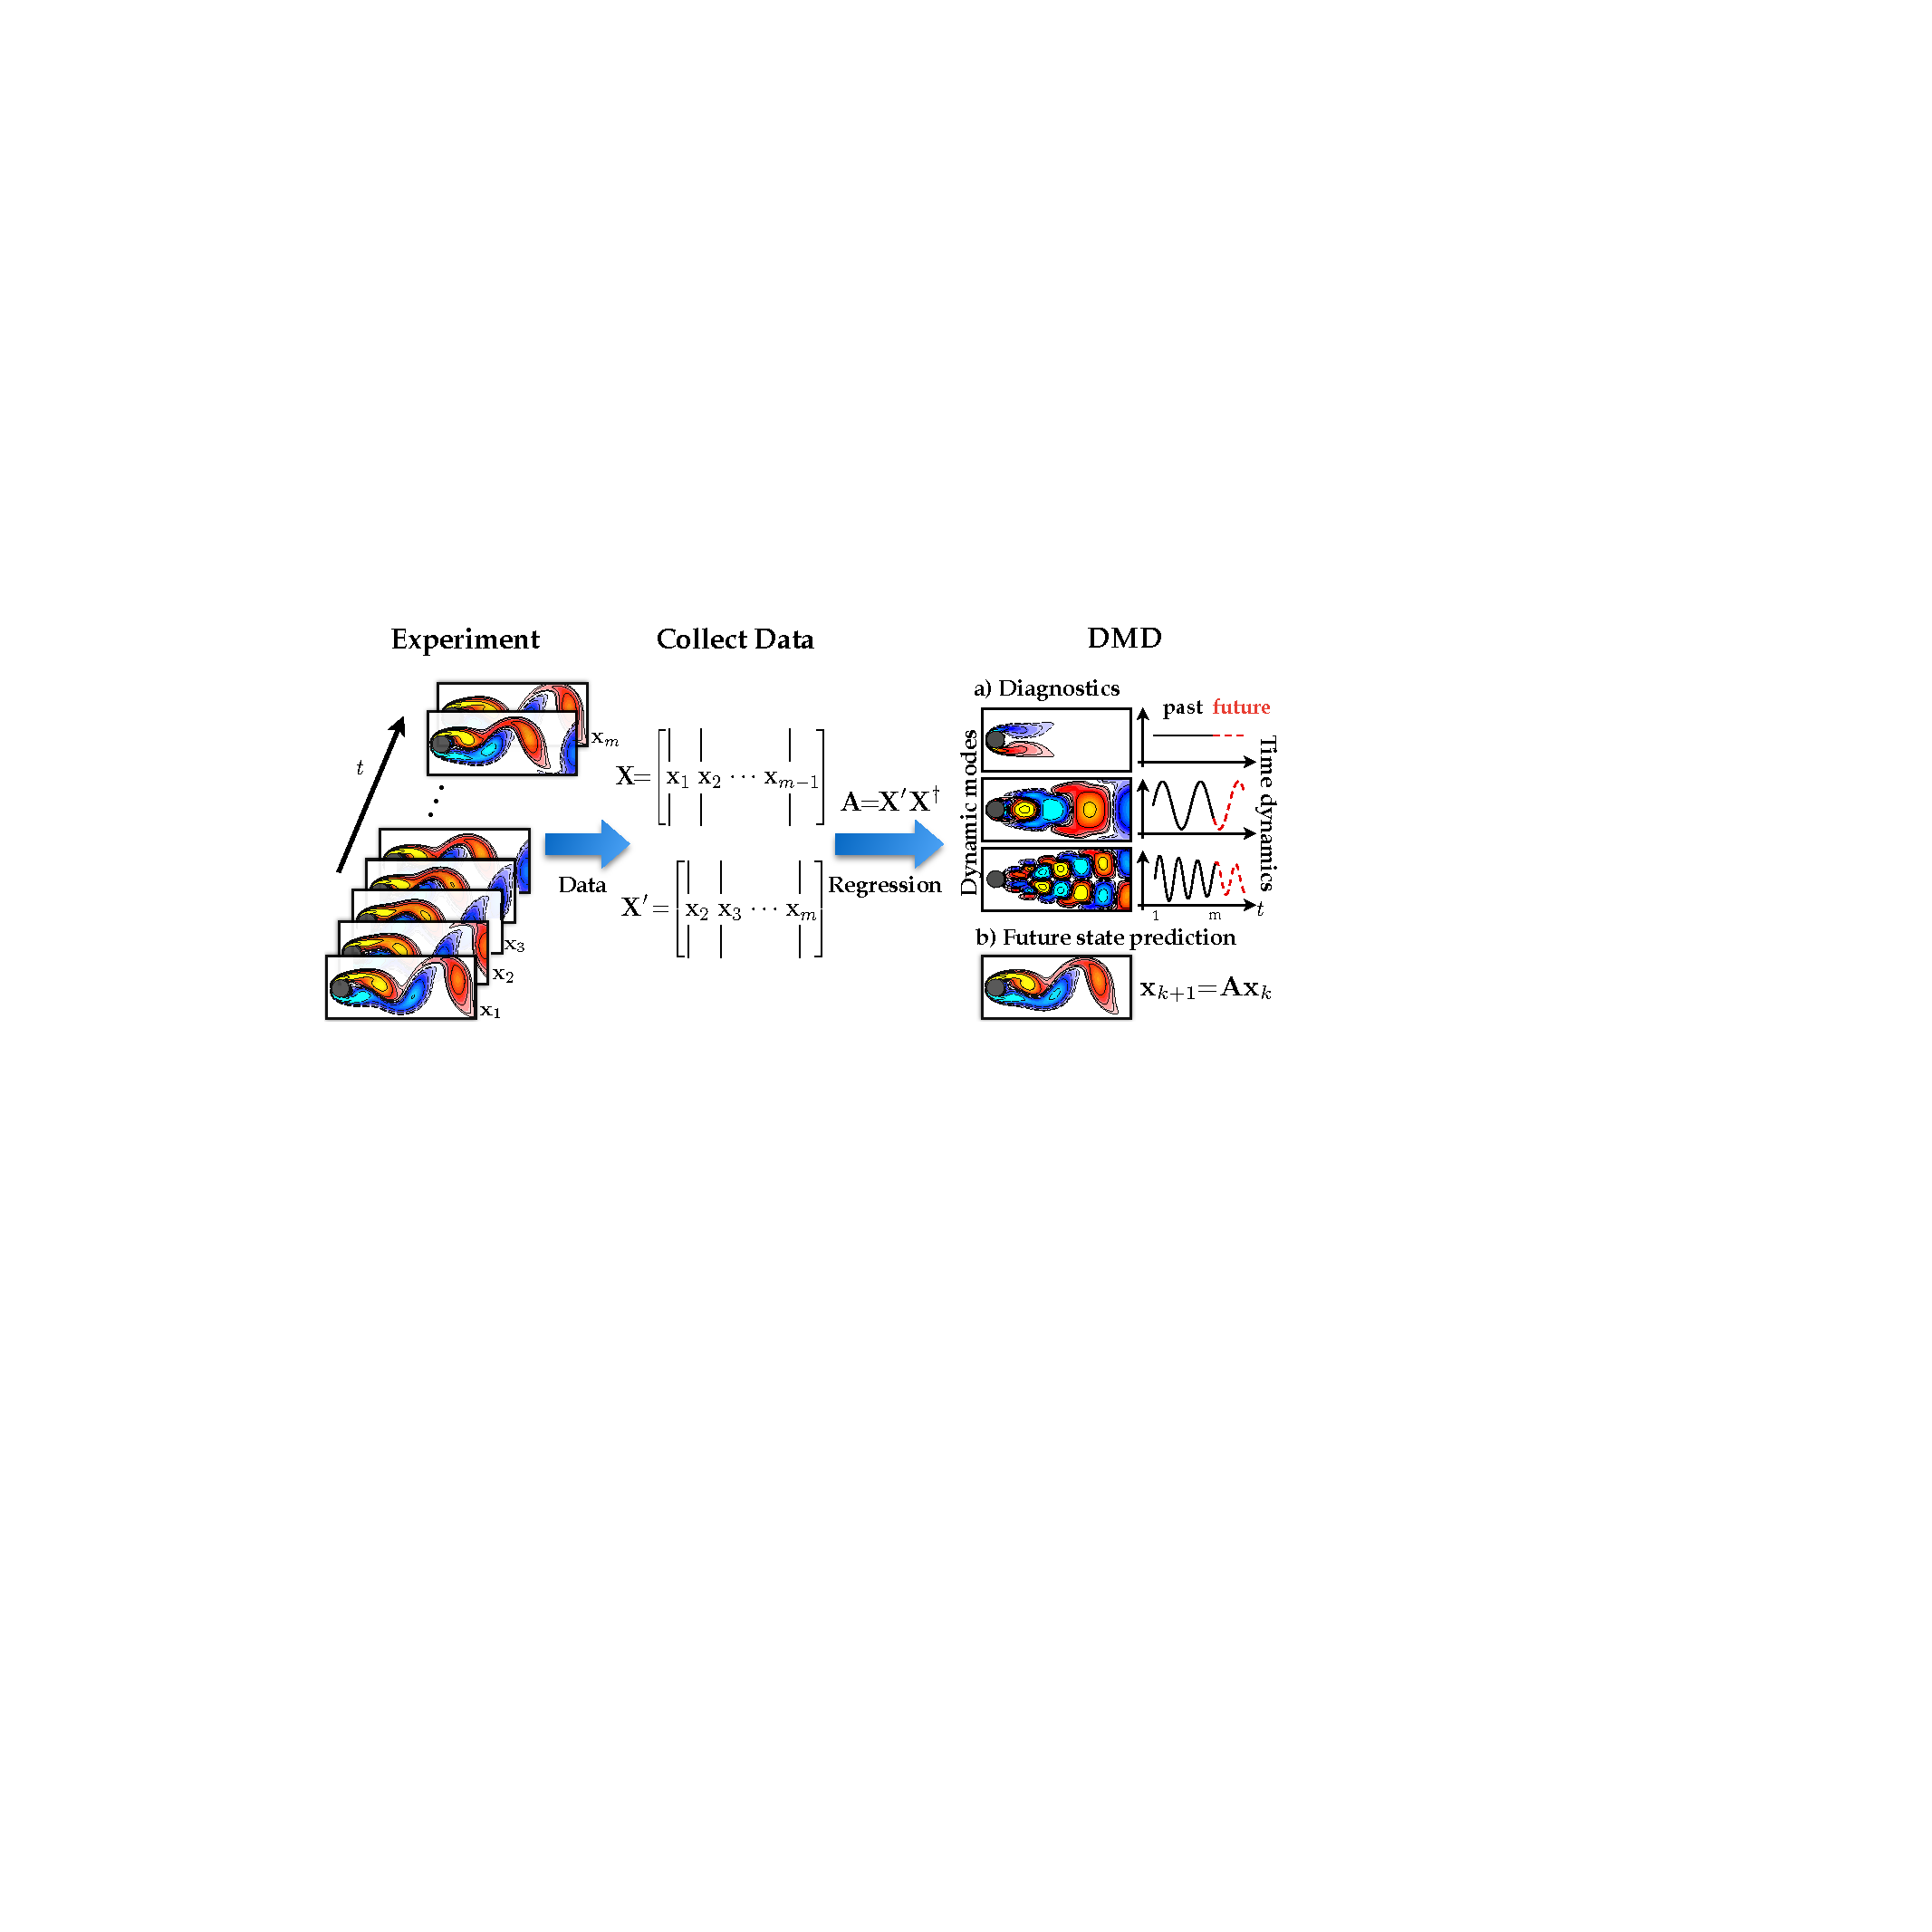
\includegraphics[width=0.8\linewidth]{fig3p1.pdf}
        \caption{\cite{brunton2021modern}}
    \end{figure}
\begin{center}
\tiny{Modern koopman theory for dynamical systems, Steven L. Brunton, 2021}
\end{center}
\end{frame}
\begin{frame}{Sparse Identification of Nonlinear Dynamics (SINDy)}
    \begin{figure}
        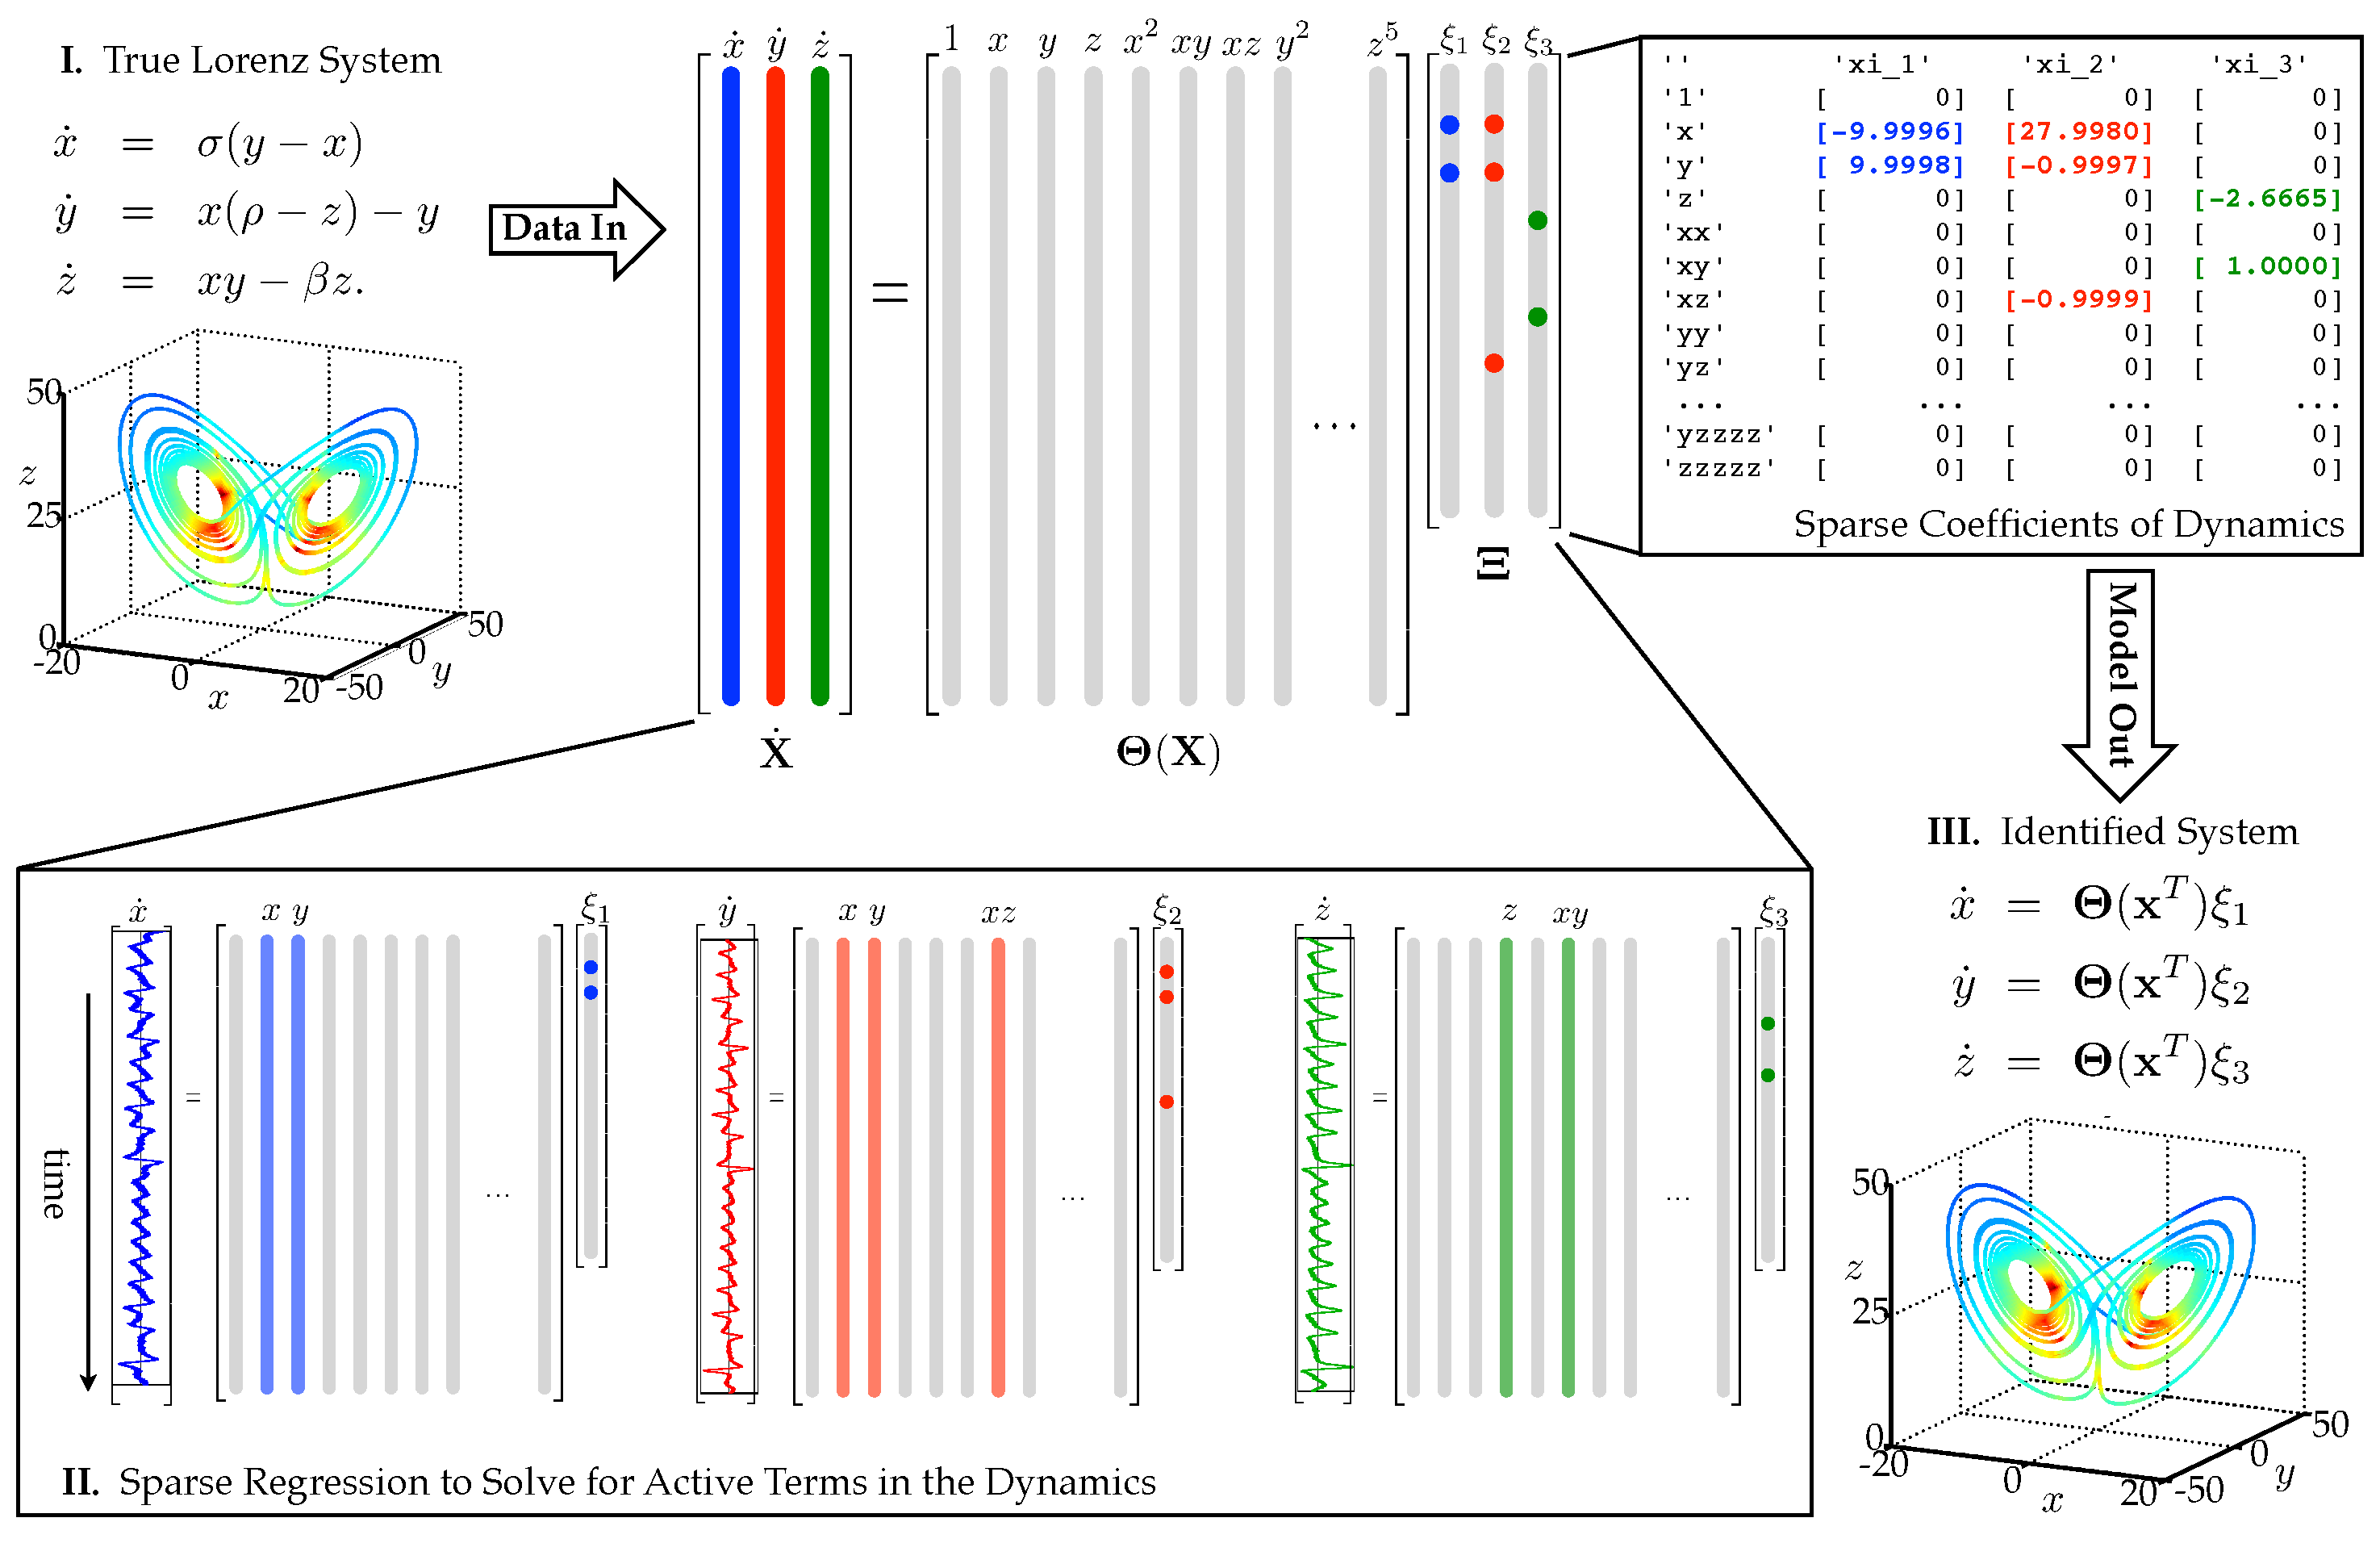
\includegraphics[width=0.5\linewidth]{FIG00_BIG4.pdf}
        \caption{\cite{brunton2021modern}}
    \end{figure}
\begin{center}
\tiny{Modern koopman theory for dynamical systems, Steven L. Brunton, 2021}
\end{center}
\end{frame}

\section{Informativity}
\begin{frame}[allowframebreaks]{Notation}{Informativity}
    \begin{itemize}
        \item Model class $\mathcal{M}$
        \item True system $\mathcal{S}$
        \item Set of data $\calD$
        \item $\Sigma_\calD$ is the set of all systems in $\calM$ that are consistent with the data $\calD$
        \item Property $\mathcal{P}$
        \item $\Sigma_\calP$ is the set of all systems in $\calM$ satisfying $\mathcal{P}$
    \end{itemize}
    %  This model class is a given set of systems that is assumed to contain the `true' system (i.e., a mathematical model of the underlying unknown physical system), denoted by $\calS$. We assume that the true system $\calS$ is not known but that we do have access to a set of data, $\calD$, which is generated by this system. As explained in the introduction, we are interested in assessing system-theoretic properties of $\calS$ and designing control laws for it from the data $\calD$.
    % Given the set of data $\calD$, we define  i.e., that could also have generated the same data. In other words,  it is impossible to distinguish the true system $\calS$ from any other system in $\Sigma_\calD$ on the basis of the given data $\calD$ alone.
    \begin{definition}[Informativity for analysis]\label{ch1:def:informativity}
        We say that the data $\calD$ are \textit{informative} for property $\calP$ if $\Sigma_\calD \subseteq\Sigma_\calP$, i.e., all systems that are consistent with the data have property $\calP$. 
    \end{definition}
    \begin{problem}[Informativity problem for analysis]\label{ch3:prob:general}
    Provide necessary and sufficient conditions on the data $\calD$ under which these data are informative for property $\calP$. 
    \end{problem}
    \begin{figure}[H]
        \centering
            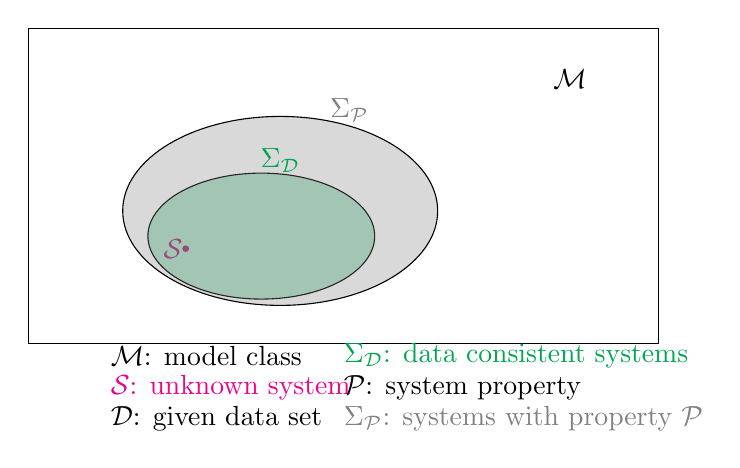
\begin{tikzpicture}[scale=0.8]
            \node[draw,rectangle,minimum width=8cm,minimum height = 4cm] (1) at (0,0) {};
            \node[] (2) at (3.6,1.7) {$\mathcal{M}$};
            \node[draw,fill,style=circle,inner sep=0pt,minimum size=2pt,color=magenta] (3) at (-2.5,-1) {};
            \node[color=magenta] (4) at (-2.7,-1) {$\mathcal{S}$};
            \node[label=right:{$\mathcal{M}$: model class}] at (-4,-2.7) {};
            \node[label=right:{\magenta{$\mathcal{S}$: unknown system}}] at (-4,-3.2) {};
            \node[label=right:{$\mathcal{D}$: given data set}] at (-4,-3.7) {};
            \node[label=right:{\green{$\Sigma_\mathcal{D}$: data consistent systems}}] at (-0.3,-2.7) {};
            \node[label=right:{\gray{$\Sigma_\mathcal{P}$: systems with property $\calP$}}] at (-0.3,-3.7) {};
            \node[label=right:{$\mathcal{P}$: system property}] at (-0.3,-3.2) {};
            \draw [fill=greenpigment,fill opacity=0.3] (-1.3,-0.8) ellipse (1.8cm and 1cm);
            \draw [fill=gray,fill opacity=0.3] (-1,-0.4) ellipse (2.5cm and 1.5cm);
            \node[] at (-1,.4) {\green{$\Sigma_\mathcal{D}$}};
            \node[] at (0.1,1.2) {\gray{$\Sigma_\mathcal{P}$}};
            %{$\mathcal{P}$}
        \end{tikzpicture}
        \caption{\cite{vanwaarde2023informativity}, The data are informative for property $\calP$ as $\Sigma_\calD \subseteq\Sigma_\calP$.}
        \label{fig:informativedata}
    \end{figure}
    \begin{center}
    \tiny{The informativity approach to data-driven analysis and control, Henk J. van Waarde, Jaap Eising, M. Kanat Camlibel, and Harry L. Trentelman, 2023}
    \end{center}
    \begin{figure}[H]
        \centering
            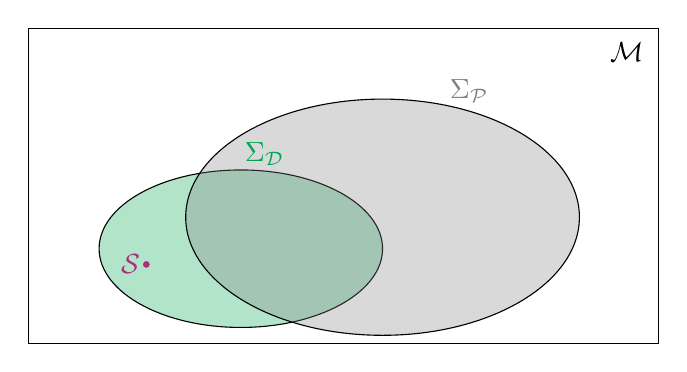
\begin{tikzpicture}[scale=1]
            \node[draw,rectangle,minimum width=8cm,minimum height = 4cm] (1) at (0,0) {};
            \node[] (2) at (3.6,1.7) {$\mathcal{M}$};
            \node[draw,fill,style=circle,inner sep=0pt,minimum size=2pt,color=magenta] (3) at (-2.5,-1) {};
            \node[color=magenta] (4) at (-2.7,-1) {$\mathcal{S}$};
            \draw [fill=greenpigment,fill opacity=0.3] (-1.3,-0.8) ellipse (1.8cm and 1cm);
            \draw [fill=gray,fill opacity=0.3] (0.5,-0.4) ellipse (2.5cm and 1.5cm);
            \node[] at (-1,.4) {\green{$\Sigma_\mathcal{D}$}};
            \node[] at (1.6,1.2) {\gray{$\Sigma_\mathcal{P}$}};
            %{$\mathcal{P}$}
        \end{tikzpicture}
        \caption{\cite{vanwaarde2023informativity}, The data are not informative for property $\calP$.}
        \label{fig:notinformativedata}
    \end{figure}
    \begin{center}
    \tiny{The informativity approach to data-driven analysis and control, Henk J. van Waarde, Jaap Eising, M. Kanat Camlibel, and Harry L. Trentelman, 2023}
    \end{center}
    \begin{definition}[Informativity for control]\label{ch1:def:par informativity}
    We say that the data $\calD$ are \textit{informative} for the control objective $\calO$ if there exists a controller $\calK$ such that $\Sigma_{\calD}(\calK) \subseteq \Sigma_{\calO}$. 
    \end{definition}
    \begin{problem}[Informativity problem for control]\label{ch1:prob:parametrized}
    Provide necessary and sufficient conditions on $\calD$ under which the data are informative for the control objective $\calO$.
    \end{problem}
    \begin{problem}[Control design problem]\label{ch1:prob:design}
    Under the assumption that the data $\calD$ are informative for the control objective $\calO$, find a controller $\calK$ such that $\Sigma_\calD (\calK) \subseteq \Sigma_{\calO}$. 
    \end{problem}

\end{frame}
\begin{frame}{Results within Informativity approach}{Informativity}
\begin{itemize}
    \item Discrete-time systems
    \item `E' refers to exact data, and `N' to noisy data
    \item State, input-state, input-state-output and input-output are denoted by `S', `IS', `ISO' and `IO', respectively
\end{itemize}
\begin{table}[H]  
\begin{center}
{\small\begin{tabular}{l|c}
Problem & Data\\
\hline
{controllability} & E-IS\\
observability & E-S\\
{stabilizability} & E-IS, N-IS\\
stability & E-S, N-S, N-IO\\
{LQR} & E-IS\\
{dissipativity} & E-ISO, N-ISO\\
{tracking and regulation} & E-IS\\
\end{tabular}}
\end{center}
\caption{Summary of results within the informativity approach to data-driven analysis and control.}
\label{tab:summary}
\end{table}
    \begin{center}
    \tiny{The informativity approach to data-driven analysis and control, Henk J. van Waarde, Jaap Eising, M. Kanat Camlibel, and Harry L. Trentelman, 2023}
    \end{center}
\end{frame}
\begin{frame}{Discrete System Framework}
    \begin{equation} \label{ch2:eq:true system once more}
    \bmx(t+1) = A_s\bmx(t) + B_s\bmu(t),
    \end{equation}
where $\bmx$ denotes the $n$-dimensional state and $\bmu$ the $m$-dimensional input.

Collect input-state data from the true system on a set of time instances $\pset{0,1,\ldots,T}$ and obtain measurements
\begin{subequations}\label{ch2:eq: UXdata}
    \begin{align}
        U_-& := \bbm u(0) & u(1) & \cdots & u(T-1)\ebm, \\
        X& := \bbm x(0) & x(1) & \cdots & x(T)\ebm.
    \end{align}
\end{subequations}
If, additionally, we define the matrices
\begin{subequations}\label{ch2:eq: def of X- X+}
    \begin{align}
        X_-& := \bbm x(0) & x(1) & \cdots & x(T-1) \ebm, \\
        X_+& := \bbm x(1) & x(2) & \cdots & x(T) \ebm,
    \end{align} 
\end{subequations}
we have $X_+=A_sX_-+B_sU_-$

Data $\calD = (U_-,X)$ and $\Sigma_\calD = \{(A_s,B_s)\}$ then
\begin{equation}\label{ch2:eq:SigmaD}
    \Sigma_\calD = \left\{ (A,B) \in \calM \mid X_+= \bbm A&B \ebm
    \begin{bmatrix}
        X_-\\U_-
    \end{bmatrix} \right\}. 
\end{equation}
\end{frame}
\section{Willems' Fundamental Lemma}
\begin{frame}[allowframebreaks]{Willems' Fundamental Lemma}
    \begin{lem}
        The data are informative for system identification if and only if the full rank condition
        \begin{equation}\label{ch2:eq:inf for sys ident} 
        \rank \begin{bmatrix} X_- \\ U_- \end{bmatrix} = n+m. 
        \end{equation}
    \end{lem}
    Consider Hankel Matrix
    \[
    H_k(u_{[0,T-1]}) := \begin{bmatrix}
            u(0)    & u(1)      & \cdots    & u(T - k) \\
            u(1)    & u(2)      & \cdots    & u(T - k +1) \\
            \vdots  & \vdots    &           & \vdots  \\
            u(k-1)  & u(k)      & \cdots    & u(T-1) 
        \end{bmatrix}.
     \]
    The input sequence $u_{[0,T-1]}$ is called \textit{persistently exciting} of order $k$ if $H_k(u_{[0,T-1]})$ has full row rank. 

    Suppose that the system is controllable and observable, and that the input sequence $u_{[0,T-1]}$ is persistently exciting of order $n+L$. Denote $X_L =\begin{bmatrix} x(0) & \cdots & x(T-L) \end{bmatrix}$. Then a consequence of Willems' fundamental lemma is that the following matrix is full rank
    \begin{equation}
    \label{stateinputHankel}
    \begin{bmatrix} X_L \\ H_L(u_{[0,T-1]}) \end{bmatrix}, 
    \end{equation}
    More generally, full row rank of \eqref{stateinputHankel} enables the identification of the system matrices $(A,B,C,D)$ up to similarity transformation if $L$ is larger than the so-called \emph{lag} of the system.
\end{frame}
\section{Dissipativity analysis}
\begin{frame}[allowframebreaks]{Dissipativity when state functions are known}{Dissipativity analysis}
    \begin{problem}
        \begin{equation}
            \begin{aligned}\label{ch5:e:lin-sys}
            \bmx(t+1)&=A \bmx(t)+B \bmu(t), \\
            \bmy(t)&=C \bmx(t)+D \bmu(t),
            \end{aligned}
        \end{equation}
    where $A\in\R^{n\times n}$, $B\in\R^{n\times m}$, $C\in\R^{p\times n}$, and $D\in\R^{p\times m}$ are given matrices. 
    \end{problem}  

    Let $S \in \S{m+p}$. The system \eqref{ch5:e:lin-sys} is said to be \emph{dissipative\/} with respect to the {\em supply rate}  
\beq\label{ch5:e:supply}
s(u,y)=\bbm u\\y\ebm^\top S \bbm u\\y\ebm
\eeq
if there exists $P \in \S{n}$ with $P \geq 0$ such that the {\em dissipation inequality\/}
\begin{equation}
\label{ch5:e:dispineq}
 \bmx(t+1)^\top P \bmx(t+1) - \bmx(t)^\top P \bmx(t) \leq s\big(\bmu(t),\bmy(t) \big) 
\end{equation} 
holds for all $t \geq 0$ and for all  trajectories $(\bmu,\bmx,\bmy): \mathbb{Z}_+ \rightarrow \mathbb{R}^{m+n+p}$ of \eqref{ch5:e:lin-sys}.  

dissipativity with respect to the supply rate \eqref{ch5:e:supply} is equivalent with the feasibility of the linear matrix inequalities $P \geq 0$ and 
\setlength\arraycolsep{2pt}
\beq\label{ch5:eq:KY_- P}
\bbm
I & 0 \\A & B
\ebm^\top
\bbm
P & 0\\0 & -P
\ebm
\bbm
I & 0 \\A & B
\ebm+
\bbm
0 & I\\C & D
\ebm^\top
S
\bbm
0 & I\\C & D
\ebm
\geq 0.
\eeq
\end{frame}
\subsection{Dissipativity from input-state-output trajectories}
\begin{frame}[allowframebreaks]{Dissipativity when state functions are unknown}{Dissipativity from input-state-output trajectories}
    \begin{problem}
        \begin{equation}
            \label{ch5:e:tru-sys}
            \begin{aligned}
            \bmx(t+1)&=A_{s} \bmx(t)+B_{s} \bmu(t),\\
            \bmy(t)&=C_{s} \bmx(t)+D_{s} \bmu(t),  \end{aligned}
        \end{equation}
    with $\bmu(t) \in \mathbb{R}^m$, $\bmx(t) \in \mathbb{R}^n$ and $\bmy(t) \in\R^{p}$ the input, state and output.

    We assume that the dimensions $m,n$ and $p$ are known, but the true system matrices $(A_{s}, B_{s},C_{s},D_{s})$ are unknown. Instead, we know finite number of input-state-output measurements of \eqref{ch5:e:tru-sys}.
    \end{problem}  
    Let $U_-,X,X_-,$ and $X_+$ be defined as the previous section and let $Y_-$ be defined in a similar way as $U_-$. Our data are now given by $\calD = (U_-,X,Y_-)$.
    \begin{equation}  \label{ch5:e:true system compatible}
    %\label{ch3:dataeq}
    \begin{bmatrix}
    X_+ \\ Y_-
    \end{bmatrix} = \begin{bmatrix}
    A_s & B_s \\ C_s & D_s
    \end{bmatrix} \begin{bmatrix}
    X_- \\ U_-
    \end{bmatrix}.
    \end{equation}
    The set of all systems that are consistent with these data is then given by: 
    \begin{equation}
    \label{ch5:eq:sigma iso}
    \Sigma_\calD = \Sigma_{(U_-,X,Y_-)}: = \left\{ (A,B,C,D) \mid \begin{bmatrix} X_+ \\ Y_- \end{bmatrix} = \begin{bmatrix} A & B \\ C & D \end{bmatrix} \begin{bmatrix} X_- \\ U_- \end{bmatrix} \right\}.
    \end{equation}
\end{frame}
\subsubsection{Noiseless data}
\begin{frame}[allowframebreaks]{Noiseless Data}{Dissipativity from input-state-output trajectories}
    We now define the  property of \emph{informativity for dissipativity} for the case of noiseless data.
    \begin{definition}[Informativity of noiseless data]\label{def:dd diss}
    The data $(U_-,X,Y_-)$ are \emph{informative for dissipativity\/} with respect to the supply rate \eqref{ch5:e:supply} if there exists a matrix $P \in \S{n}$, $P \geq0$, such that the LMI \eqref{ch5:eq:KY_- P} holds for every system $(A,B,C,D) \in \Sigma_{(U_-,X,Y_-)}$. 
    \end{definition}
    Note that this definition of informativity for dissipativity requires the systems in $\Sigma_{(U_-,X,Y_-)}$ to be dissipative with a \emph{common} storage function. 

    We will impose the following assumption on the inertia of $S = (\rho_-, \rho_0, \rho_+)=(p,0,m)$. % These are the number of negative, zero, and positive eigenvalues of $S$ respectively.
    % This assumption is satisfied, for example, for the positive-real and bounded-real case.  Indeed, in the positive-real case we have that $m = p$ and
    
    For positive-real case,
    $S = \begin{bmatrix}
    0 & I_m \\ I_m & 0
    \end{bmatrix},
    $
    so that $\In(S) = (m,0,m)$.

    For bounded-real case,
    $
    S = \begin{bmatrix}
    \gamma^2 I_m & 0 \\ 0 & -I_p
    \end{bmatrix}
    $
    for some $\gamma > 0$, which implies that $\In(S)=(p,0,m)$. 
    \begin{theorem}[Informativity of noiseless data] \label{ch5:th:info diss}
    Assuming that $\In(S)=(p,0,m)$. Then the data $(U_- ,X,Y_- )$ are informative for dissipativity with respect to the supply rate \eqref{ch5:e:supply} if and only if they are informative for system identification
    and there exists $P=P^\top \geq0$ such that
    \beq\label{ch5:e:exact cond2}
    \bbm
    X_-\\X_+
    \ebm^\top
    \bbm
    P & 0\\0 & -P
    \ebm
    \bbm
    X_-\\X_+
    \ebm+
    \bbm
    U_- \\Y_- 
    \ebm^\top
    S
    \bbm
    U_- \\Y_- 
    \ebm
    \geq 0.
    \eeq
    \end{theorem}
\end{frame}
\subsubsection{Noisy data}
\begin{frame}[allowframebreaks]{Noisy Data}{Dissipativity from input-state-output trajectories}
\begin{problem}
    \begin{equation}
        \begin{aligned}
        \bmx(t+1)&=A_{s} \bmx(t)+B_{s} \bmu(t)  + \bmw(t),\\
        \bmy(t)&=C_{s} \bmx(t)+D_{s} \bmu(t) + \bmz(t),  \end{aligned}
    \end{equation}
    where $\bmu(t) \in \mathbb{R}^m$, $\bmx(t) \in \mathbb{R}^n$ and $\bmy(t) \in\R^{p}$ are the input, state and output.

    The dimensions $m,n$ and $p$ are assumed to be known. 
    
    The noise terms $\bmw$ and $\bmz$ are unknown, so $w(0),w(1),\dots,w(T-1)$ and  $z(0),z(1),\dots,z(T-1)$ are not measured, and are therefore not part of the data. 
\end{problem}
\begin{definition}[Noise model] \label{ch5:assumption on noise samples}
The noise samples,
%$w(0),w(1),\dots,w(T-1)$ and $z(0),z(1),\dots,z(T-1)$, 
collected in the real $(n + p) \times T$ matrix 
$$
V_- := \bbm w(0) & w(1) & \cdots & w(T-1) \\  z(0) & z(1)  & \cdots & z(T-1)    \ebm
$$
satisfy the quadratic matrix inequality
\begin{equation} 
    \label{ch5:asnoise}
    \begin{bmatrix}
    I \\ V_-^\top 
    \end{bmatrix}^\top 
    \Phi
    \begin{bmatrix}
    I \\ V_-^\top 
    \end{bmatrix} \geq 0,
\end{equation}
\end{definition}
\begin{definition}    
where $\Phi \in \S{n +p + T}$ is a given partitioned matrix 
\begin{equation} \label{ch5:eq:Phi}
\Phi = \bbm \Phi_{11}  & \Phi_{12} \\ \Phi_{21} & \Phi_{22} \ebm
\end{equation}
with $\Phi_{11} \in \S{n + p}$, $\Phi_{12} \in \mathbb{R}^{(n + p) \times T}$, $\Phi_{21} = \Phi_{12}^\top$ and $\Phi_{22} \in \S{T}$.

We assume that $\calZ_T(\Phi)$ is nonempty and convex.\footnote{\tiny{This assumption comes from Quadratic matrix inequalities results.}}

We have that $V_-$ satisfies \eqref{ch5:asnoise} if and only if $V_-^\top \in \calZ_T(\Phi)$ where
\begin{equation} \label{ch0:e:Zr}
\calZ_{T}(\Phi):=\left\{ Z\in\R^{T\times q} \mid \bbm I_q\\Z\ebm^\top\Phi\bbm I_q\\Z\ebm\geq 0\right\},
\end{equation}
\end{definition}
\begin{equation} \label{ch5:def:SigmaD}
\Sigma_{\calD} = \left \lbrace (A,B,C,D) \! \mid \! \left(\begin{bmatrix} X_+\\Y_-  \end{bmatrix} \!-\! \begin{bmatrix} A&B\\
C&D\end{bmatrix}\!\begin{bmatrix}X_-\\ U_-  \end{bmatrix}\right)^\top \!\in\!\calZ_T(\Phi)  \right \rbrace.
\end{equation}
We assume that the data have been obtained from the unknown system, i.e., $(A_s,B_s,C_s,D_s) \in \Sigma_{\calD}$. Therefore, $\Sigma_{\calD}$ is nonempty. Define
\begin{equation} \label{ch5:eq:bigN}
N\!:= \!\begin{pmat}[{|}]
N_{11} & N_{12} \cr\- N_{12}^\top & N_{22} \cr
\end{pmat} \! = \! \left[\begin{array}{c|c}
I & \begin{array}{c}
X_+\\Y_- 
\end{array}
\\\hline
0 & \begin{array}{c}
-X_-\\-U_- 
\end{array}
\end{array}\right]
\!\!
\bbm
\Phi_{11} & \Phi_{12}\\
\Phi_{21} & \Phi_{22}
\ebm\!\!
\left[\begin{array}{c|c}
I & \begin{array}{c}
X_+\\Y_- 
\end{array}
\\\hline
0 & \begin{array}{c}
-X_-\\-U_- 
\end{array}
\end{array}\right]^\top\!\!.
\end{equation}
Note that $(A,B,C,D)\in \Sigma_{\calD}$ if and only if
\beq \label{ch5:e:char N2 model}
\bbm
I\\\hline\\[-3mm]
\begin{matrix}
A^\top & C^\top\!\\
B^\top & D^\top\!
\end{matrix}
\ebm^\top\!\! 
N
\bbm
I\\\hline\\[-3mm]
\begin{matrix}
A^\top & C^\top\!\\
B^\top & D^\top\!
\end{matrix}
\ebm
\geq 0.
\qquad\equiv\qquad
\bbm
A^\top & C^\top\!\\
B^\top & D^\top\!
\ebm \in \calZ_{n + m}(N).
\eeq
\end{frame}
\begin{frame}[allowframebreaks]{Informativity of noisy data}{Dissipativity from input-state-output trajectories}
    \begin{definition}[Informativity of noisy data]\label{ch5:def:info diss noisy}
    The noisy input-state-output data $(U_-,X,Y_-)$ are \emph{informative for dissipativity\/} with respect to the supply rate \eqref{ch5:e:supply} if there exists a matrix $P\geq 0$ such that the LMI \eqref{ch5:eq:KY_- P} holds for all systems $(A,B,C,D)\in\Sigma_{\calD}$. 
    \end{definition}
    \begin{lem}[Necessity of full row rank condition] \label{ch5:lem:necc noisy case} 
    Assuming that $\In(S)=(p,0,m)$. If the data $(U_- ,X,Y_- )$ are informative for dissipativity with respect to the supply rate \eqref{ch5:e:supply} then \ref{ch2:eq:inf for sys ident} holds.
    \end{lem}
    \begin{lem}[Necessity of positive definite storage]
    \label{ch5:lem:P>0}
    Suppose that $\In(S)=(p,0,m)$ and that $N \schur N_{22} >0$. If $P \geq 0$ satisfies the dissipation inequality \eqref{ch5:eq:KY_- P} for all $(A,B,C,D) \in \Sigma_{\calD}$ then $P > 0$. 
    \end{lem}
    Our next step is to partition 
    \begin{equation} \label{ch5:eq:partitionS}
    S=\bbm F & G\\G^\top & H\ebm,
    \end{equation}
    where  $F\in\R^{m\times m}$, $G\in\R^{m\times p}$, $H\in\R^{p\times p}$. For any $P \geq 0$ define
    \begin{equation} \label{ch5:eq:partitionM}
    M:=\bbm
    P & 0 & 0 & 0\\
    0 & F & 0 & G\\
    0 & 0 & -P & 0\\
    0 & G^\top & 0 & H
    \ebm.
    \end{equation}
    Then the system $(A,B,C,D)$ can be seen to satisfy the dissipation inequality \eqref{ch5:eq:KY_- P} if and only if  
    \begin{equation}
    \label{ch5:eq:eqM1}
    \sysone^\top\!\! M \sysone \geq 0
    \end{equation} 
    \begin{theorem}[Matrix S-lemma \cite{9781292}]
    \label{t:nonstrictS-lemma}
    Let $M,N \in \mathbb{S}^{q+r}$. If there exists a real $\alpha \geq 0$ such that $M - \alpha N \geq 0$, then $\calZ_r(N) \subseteq \calZ_r(M)$. Next, assume that $N \in \bpi_{q,r}$ and $N$ has at least one positive eigenvalue. Then $\calZ_r(N) \subseteq \calZ_r(M)$ if and only if there exists a real $\alpha \geq 0$ such that $M-\alpha N \geq 0$. 
    \end{theorem}
    \begin{lem}[Dualization of dissipation inequality \cite{vanwaarde2023informativity}]\label{ch5:lem:diss dual}
    Let  $P > 0$ and let $(A,B,C,D)$ be any system with input dimension $m$, state space dimension $n$ and output dimension $p$. Assume that $\In(S) = (p,0,m)$. Define
    \begin{equation}
    \label{ch5:eq:Shat}
     \hat{S}:=\begin{bmatrix} 0&-I_p\\
     I_m&0 \end{bmatrix} S\inv \begin{bmatrix} 0&-I_m\\I_p&0 \end{bmatrix}.
    \end{equation}
    Then we have
    \begin{equation}
    \label{ch5:eq:eqL1}
    \begin{bmatrix}
    I&0\\
    A&B
    \end{bmatrix}^\top\!\!\begin{bmatrix}
    P&0\\
    0&-P
    \end{bmatrix}\begin{bmatrix}
    I&0\\
    A&B
    \end{bmatrix}+\begin{bmatrix}
    0&I\\
    C&D
    \end{bmatrix}^\top\!\! S \begin{bmatrix}
    0&I\\
    C&D
    \end{bmatrix}\geq 0
    \end{equation}
    if and only if 
    \begin{align}\label{ch5:eq:L2}
    \begin{bmatrix}
    I&0 \!\\
    A^\top&C^\top\!
    \end{bmatrix}^\top\!\!\!\begin{bmatrix}
    P^{-1}&0\\
    0&-P^{-1}
    \end{bmatrix}\!\!\!
    \begin{bmatrix}
    I&0\!\! \\
    A^\top&C^\top\!\!
    \end{bmatrix}\!\!+\!\!\begin{bmatrix}
    0&I \!\! \\
    B^\top&D^\top \!\!
    \end{bmatrix}^\top\!\!\!\! \hat{S}\!\! \begin{bmatrix}
    0&I \!\! \\
    B^\top&D^\top \!\!
    \end{bmatrix} \!\!\geq\! 0.
    \end{align}
    \end{lem}
    \bthe[Informativity of noisy data] \label{ch5:t:noise 1}
    Suppose that the data $(U_-,X,Y_-)$ are collected from system \ref{ch2:eq:SigmaD} with noise as in Assumption~\ref{ch5:assumption on noise samples}.
    In addition, assume that $\In(S) = (p,0,m)$ and that the data $(U_- ,X,Y_- )$ are such that $N \schur N_{22} >0$. Partition 
    \begin{equation} \label{ch5:eq:partition of Sinv}
    -S\inv = \begin{bmatrix}
    \hatF&\hatG\\
    \hatG^\top  &\hatH
    \end{bmatrix},
    \end{equation}
    where $\hatF=\hatF^\top \in\R^{m\times m}$, $\hatG\in\R^{m\times p}$, and $\hatH=\hatH^\top \in\R^{p\times p}$. 

    Then the data are informative for dissipativity with respect to the supply rate \eqref{ch5:e:supply} if and only if there exist a real $n \times n$ matrix $Q \in \S{n}$, $Q >0$ and a scalar $\alpha\geq 0$ such that 
    \begin{equation}
    \begin{bmatrix}
        \! Q & \!0\! & \!0\! & 0 \!\!\! \\
        \! 0 & \!\hatH\! & \!0\! &-\hatG^\top \!\!\! \\
       \! 0 & \!0\! & \!-Q\! & 0 \!\!\! \\
       \! 0 & \!-\hatG\! & \!0\! & \hatF \!\!\!
        \end{bmatrix} \!-\! \alpha\!\!
        \None
         \!\!\!\!\geq\! 0. \label{ch5:eq:LMI2}
    \end{equation}
    % In that case $P : = Q^{-1}$ is a common storage function for all systems consistent with the data.
    \ethe
\end{frame}
\subsection{Dissipativity from input-output trajectories}
\begin{frame}[allowframebreaks]{Dissipativity when state functions are unknown}{Dissipativity from input-output trajectories}
    \begin{problem}
        \begin{equation}
            \begin{aligned}
            \bmx(t+1)&=A_{s} \bmx(t)+B_{s} \bmu(t),\\
            \bmy(t)&=C_{s} \bmx(t)+D_{s} \bmu(t),  \end{aligned}
        \end{equation}
    with $\bmu(t) \in \mathbb{R}^m$, $\bmx(t) \in \mathbb{R}^n$ and $\bmy(t) \in\R^{p}$ the input, state and output.

    We assume that the dimensions $m,n$ and $p$ are known, but the true system matrices $(A_{s}, B_{s},C_{s},D_{s})$ are unknown. Instead, we know finite number of input-state-output measurements of \eqref{ch5:e:tru-sys}.
    \end{problem}  
    Let $U_-,$ be defined as the previous section and let $Y_-$ be defined in a similar way as $U_-$. Our data are now given by $\calD = (U_-,Y_-)$.
    % \begin{equation}  \label{ch5:e:true system compatible}
    % %\label{ch3:dataeq}
    % \begin{bmatrix}
    % X_+ \\ Y_-
    % \end{bmatrix} = \begin{bmatrix}
    % A_s & B_s \\ C_s & D_s
    % \end{bmatrix} \begin{bmatrix}
    % X_- \\ U_-
    % \end{bmatrix}.
    % \end{equation}
    % The set of all systems that are consistent with these data is then given by: 
    % \begin{equation}
    % \label{ch5:eq:sigma iso}
    % \Sigma_\calD = \Sigma_{(U_-,X,Y_-)}: = \left\{ (A,B,C,D) \mid \begin{bmatrix} X_+ \\ Y_- \end{bmatrix} = \begin{bmatrix} A & B \\ C & D \end{bmatrix} \begin{bmatrix} X_- \\ U_- \end{bmatrix} \right\}.
    % \end{equation}
\end{frame}
\begin{frame}{Assumptions}{Dissipativity from input-output trajectories}
    \begin{definition}
    The lag $\underline{l}$ of system~\eqref{ch5:e:tru-sys} is the smallest integer $l \in \mathbb{N}_{+}$ such that the observability matrix given by 
    \begin{align*}
    \mathcal{O}_l \coloneqq \begin{bmatrix} C \\ CA \\ \vdots \\ CA^{l-1}
    \end{bmatrix}
    \end{align*}
    has rank $n$.
    \label{def:lag}
    \end{definition}
    The upper bound on the lag of the system $$\underline{l} \leq l$$
\end{frame}
\subsubsection{Noiseless Data}
\begin{frame}[allowframebreaks]{Noiseless Data}{Dissipativity from input-output trajectories}
    \begin{lem}
    \label{lem:extended}
    Let $l \geq \underline{l}$. Then there exists a system $\widetilde{G}$ with matrices $\widetilde{A},\widetilde{B},\widetilde{C},\widetilde{D}$ which can explain the data $\{u_k\}_{k=0}^{N-1}$, $\{y_k\}_{k=0}^{N-1}$, i.e., there exists $\xi_0$ such that for $k=0,\dots,N-1$,
    \begin{align}\label{eq:sys_stacked}
    \xi_{k+1} = \widetilde{A} \xi_k + \widetilde{B} u_k, \quad
    y_k = \widetilde{C} \xi_k + \widetilde{D} u_k,
    \end{align}
    where the extended state is defined by
    \begin{align*}
    {
    \xi_{k} = \begin{bmatrix} u_{k-l}^\top & u_{k-l+1}^\top & \cdots & u_{k-1}^\top & y_{k-l}^\top & y_{k-l+1}^\top & \cdots & y_{k-1}^\top \end{bmatrix}^\top.}
    \end{align*} 
    \end{lem}
    \begin{proof}
    The input-output behavior of the system $G$ in \eqref{ch5:e:tru-sys} over $l$ steps can be written as \eqref{eq:input-output},
    \begin{align}
    \begin{bmatrix} y_{k-l} \\ y_{k-l+1} \\ \vdots \\ y_{k-1} \end{bmatrix} = \underbrace{\begin{bmatrix} C_s \\ C_sA_s \\ \vdots \\ C_sA_s^{l-1} \end{bmatrix}}_{\mathcal{O}_l} x_{k-l} + 
    \underbrace{\begin{bmatrix} 
    D_s & 0 & & \dots & 0 & 0 \\
    C_sB_s & D _s& & \dots & 0 & 0 \\
    \vdots & \ddots & \ddots&\ddots&\ddots&\vdots \\
    C_sA_s^{l-2}B_s & C_sA_s^{l-3}B_s &\dots & C_sA_sB_s & C_sB_s &D_s
    \end{bmatrix} }_R
    \begin{bmatrix} u_{k-l} \\ u_{k-l+1} \\ \vdots \\ u_{k-1} \end{bmatrix}
    \label{eq:input-output}
    \end{align}
    \proofbreak
    which yields with the introduced matrix notation
    %
    \begin{align*}
    \begin{bmatrix} 
    -R & I
    \end{bmatrix} \xi_k = \mathcal{O}_l x_k.
    \end{align*}
    %Note that with
    Using the definition of the lag, we know that $\mathcal{O}_l$ has full column rank, and hence, there exists a left-inverse $\mathcal{O}_l^{-1}$ (which has full row rank) such that
    \begin{align}
    \underbrace{\mathcal{O}_l^{-1} \begin{bmatrix} 
    -R & I
    \end{bmatrix}}_{K} \xi_k = x_k.
    \label{eq:trafo}
    \end{align}
    % \proofbreak

    % The general system description from \eqref{ch5:e:tru-sys} yields
    \begin{align*}
    y_{k} = C_s A_s^l x_{k-l} + \begin{bmatrix} C_sA_s^{l-1} B_s & \dots & C_sB_s \end{bmatrix} \begin{bmatrix} u_{k-l} \\ \vdots \\ u_{k-1} \end{bmatrix}.
    \end{align*}
    % Together with $K$, %$T=\mathcal{O}_l^{-1}\begin{bmatrix}-R I\end{bmatrix}$
    % this leads to,
    \proofbreak
    \begin{align}
    \begin{split}
    \label{eq:extended_sys}
    \underbrace{\begin{bmatrix} u_{k-l+1} \\ \vdots \\ u_{k-1} \\ u_{k} \\ y_{k-l+1} \\ \vdots \\ y_{k-1} \\ y_{k}  \end{bmatrix}}_{\xi_{k+1}} &= \underbrace{\begin{bmatrix} 
    0 & I & \dots & 0 & 0 &  0& \dots &0 \\
    \vdots & \ddots & \ddots&\ddots& \vdots & & \ddots&\vdots \\
    0 & 0 & \dots & I & 0& 0&  \dots & 0 \\
    0 & 0 & \dots & 0 & 0 & 0&  \dots & 0 \\
    0 & 0 & \dots & 0 & 0& I& \dots &0 \\
    \vdots & \ddots & \ddots&\vdots&\vdots & & \ddots&\vdots \\
    0 & 0 & \dots & 0 & 0& 0&  \dots & I \\
    C_sA_s^{l-1}B_s & \dots & \dots & C_sB_s & 0 & 0 & \dots &  0 \\
    \end{bmatrix} + \begin{bmatrix} 0 \\ \vdots \\ 0\\ 0 \\ 0 \\ \vdots \\ 0 \\ C_s A_s^l T \end{bmatrix} }_{\widetilde{A}} \underbrace{\begin{bmatrix} u_{k-l} \\ u_{k-l+1} \\ \vdots \\ u_{k-1} \\ y_{k-l} \\ y_{k-l+1} \\ \vdots \\ y_{k-1} \end{bmatrix}}_{\xi_{k}} + \underbrace{\begin{bmatrix} 0 \\ \vdots \\ 0 \\ I \\ 0 \\ \vdots \\ 0 \\ D_s  \end{bmatrix}}_{\widetilde{B}} u_{k} \\
    y_k &= \underbrace{\begin{bmatrix} 0 & \dots & 0 & I \end{bmatrix} \tilde{A}}_{\tilde{C}} \xi_k + \underbrace{D}_{\tilde{D}} u_k
    \end{split} 
    \end{align}
    % This proves that $(\tilde{A}, \tilde{B}, \tilde{C}, \tilde{D})$ can explain the input-output trajectory. 
    \end{proof} 
\end{frame}
\begin{frame}{Noiseless Data}{Dissipativity from input-output trajectories}
    \begin{theorem}[Informativity of noiseless data] \label{ch5:th:info diss}
    Assuming that $\In(S)=(p,0,m)$ and the lag of the system $\underline{l}\leq l$. Then the data $(U_-,Y_- )$ are informative for dissipativity with respect to the supply rate \eqref{ch5:e:supply} if and only if they are informative for system identification
    and there exists $P=P^\top \geq0$ such that
    \beq\label{ch5:e:exact cond3}
    \bbm
    \Xi_-\\\Xi_+
    \ebm^\top
    \bbm
    P & 0\\0 & -P
    \ebm
    \bbm
    \Xi_-\\\Xi_+
    \ebm+
    \bbm
    U_{\Xi_-} \\Y_{\Xi_-} 
    \ebm^\top
    S
    \bbm
    U_{\Xi_-} \\Y_{\Xi_-} 
    \ebm
    \geq 0.
    \eeq
    where $\xi_{k} = \begin{bmatrix} u_{k-l}^\top & u_{k-l+1}^\top & \cdots & u_{k-1}^\top & y_{k-l}^\top & y_{k-l+1}^\top & \cdots & y_{k-1}^\top \end{bmatrix}^\top$ and, 
    \begin{align*}
    \Xi_- &\coloneqq \begin{bmatrix} \xi_l & \xi_{l+1} & \cdots & \xi_{T-1} \end{bmatrix}, \\
    \Xi_+ &\coloneqq \begin{bmatrix} \xi_{l+1} & \xi_{l+2} & \cdots & \xi_{T} \end{bmatrix}, \\ 
    Y_{\Xi_-} &\coloneqq \begin{bmatrix} y_{l} & y_{l+1} & \cdots & y_{T-1} \end{bmatrix}, \\
    U_{\Xi_-} &\coloneqq \begin{bmatrix} u_{l} & u_{l+1} & \cdots & u_{T-1} \end{bmatrix},
    \end{align*}
    \end{theorem}
\end{frame}
\appendix
\subsubsection{Noisy Data}
\begin{frame}[allowframebreaks]{Noisy Data}{Dissipativity from input-output trajectories}
    \begin{problem}
        \begin{equation}
            \begin{aligned}
            \bmx(t+1)&=A_{s} \bmx(t)+B_{s} \bmu(t)  + \bmw(t),\\
            \bmy(t)&=C_{s} \bmx(t)+D_{s} \bmu(t) + \bmz(t),  \end{aligned}
        \end{equation}
        where $\bmu(t) \in \mathbb{R}^m$, $\bmx(t) \in \mathbb{R}^n$ and $\bmy(t) \in\R^{p}$ are the input, state and output.

        The dimensions $m,n$ and $p$ are assumed to be known. 
        
        The noise terms $\bmw$ and $\bmz$ are unknown, so $w(0),w(1),\dots,w(T-1)$ and  $z(0),z(1),\dots,z(T-1)$ are not measured, and are therefore not part of the data. 
    \end{problem}
\end{frame}
\begin{frame}[allowframebreaks]{Informativity of noisy data using the complete system}{Dissipativity from input-output trajectories}
    Using \ref{eq:extended_sys}, we define
    \begin{definition}[Noise model] \label{ch5:assumption on noise samples}
    The noise samples,
    %$w(0),w(1),\dots,w(T-1)$ and $z(0),z(1),\dots,z(T-1)$, 
    collected in the real $(n+p) \times (T-l)$ matrix  %((m + p)\cdot l
    $$
    V_- := \bbm \tilde{w}(l) & \tilde{w}(l+1) & \cdots & \tilde{w}(T-1) \\  \tilde{z}(l) & \tilde{z}(l+1)  & \cdots & \tilde{z}(l-1)    \ebm
    $$
    satisfy the quadratic matrix inequality
    \begin{equation} 
        \label{ch5:asnoise}
        \begin{bmatrix}
        I \\ V_-^\top 
        \end{bmatrix}^\top 
        \Phi
        \begin{bmatrix}
        I \\ V_-^\top 
        \end{bmatrix} \geq 0,
    \end{equation}
    \end{definition}
    \begin{definition}    
    where $\Phi \in \S{(n+p) + (T-l)}$ is a given partitioned matrix 
    \begin{equation} \label{ch5:eq:Phi}
    \Phi = \bbm \Phi_{11}  & \Phi_{12} \\ \Phi_{21} & \Phi_{22} \ebm
    \end{equation}
    with $\Phi_{11} \in \S{n+p}$, $\Phi_{12} \in \mathbb{R}^{(n+p) \times (T-l)}$, $\Phi_{21} = \Phi_{12}^\top$ and $\Phi_{22} \in \S{(T-l)}$.

    We assume that $\calZ_T(\Phi)$ is nonempty and convex.\footnote{\tiny{This assumption comes from Quadratic matrix inequalities results.}}

    We have that $V_-$ satisfies \eqref{ch5:asnoise} if and only if $V_-^\top \in \calZ_T(\Phi)$ where
    \begin{equation} \label{ch0:e:Zr}
    \calZ_{T}(\Phi):=\left\{ Z\in\R^{T\times q} \mid \bbm I_q\\Z\ebm^\top\Phi\bbm I_q\\Z\ebm\geq 0\right\},
    \end{equation}
    \end{definition}
    \begin{equation} \label{ch5:def:SigmaD}
    \Sigma_{\calD} = \left \lbrace (A,B,C,D) \! \mid \! \left(\begin{bmatrix} \Xi_+\\Y_{\Xi_-}  \end{bmatrix} \!-\! \begin{bmatrix} A&B\\
    C&D\end{bmatrix}\!\begin{bmatrix}\Xi_-\\ U_{\Xi_-}  \end{bmatrix}\right)^\top \!\in\!\calZ_T(\Phi)  \right \rbrace.
    \end{equation}
    We assume that the data have been obtained from the unknown system, i.e., $(A_s,B_s,C_s,D_s) \in \Sigma_{\calD}$. Therefore, $\Sigma_{\calD}$ is nonempty. Define
    \begin{equation} \label{ch5:eq:bigN}
    N\!:= \!\begin{pmat}[{|}]
    N_{11} & N_{12} \cr\- N_{12}^\top & N_{22} \cr
    \end{pmat} \! = \! \left[\begin{array}{c|c}
    I & \begin{array}{c}
    \Xi_+\\Y_{\Xi_-} 
    \end{array}
    \\\hline
    0 & \begin{array}{c}
    -\Xi_-\\-U_{\Xi_-} 
    \end{array}
    \end{array}\right]
    \!\!
    \bbm
    \Phi_{11} & \Phi_{12}\\
    \Phi_{21} & \Phi_{22}
    \ebm\!\!
    \left[\begin{array}{c|c}
    I & \begin{array}{c}
    \Xi_+\\Y_{\Xi_-} 
    \end{array}
    \\\hline
    0 & \begin{array}{c}
    -\Xi_-\\-U_{\Xi_-} 
    \end{array}
    \end{array}\right]^\top\!\!.
    \end{equation}
    Note that $(A,B,C,D)\in \Sigma_{\calD}$ if and only if
    \beq \label{ch5:e:char N2 model}
    \bbm
    I\\\hline\\[-3mm]
    \begin{matrix}
    A^\top & C^\top\!\\
    B^\top & D^\top\!
    \end{matrix}
    \ebm^\top\!\! 
    N
    \bbm
    I\\\hline\\[-3mm]
    \begin{matrix}
    A^\top & C^\top\!\\
    B^\top & D^\top\!
    \end{matrix}
    \ebm
    \geq 0.
    \qquad\equiv\qquad
    \bbm
    A^\top & C^\top\!\\
    B^\top & D^\top\!
    \ebm \in \calZ_{n + m}(N).
    \eeq
    
    \bthe[Informativity of noisy data] \label{ch5:t:noise 1}
    Suppose that the data $(U_-,Y_-)$ are collected from system \ref{ch2:eq:SigmaD} with noise% as in Assumption~\ref{ch5:assumption on noise samples}.
    In addition, assume that $\In(S) = (p,0,m)$ and that the data $(U_- ,X,Y_- )$ are such that $N \schur N_{22} >0$. Partition the equivalent supply rate $\tilde{S}$,
    \begin{equation} \label{ch5:eq:partition of Sinv}
    -\tilde{S}\inv = \begin{bmatrix}
    \hatF&\hatG\\
    \hatG^\top  &\hatH
    \end{bmatrix},
    \end{equation}
    % where $\hatF=\hatF^\top \in\R^{m\times m}$, $\hatG\in\R^{m\times p}$, and $\hatH=\hatH^\top \in\R^{p\times p}$. 
    Then the data are informative for dissipativity with respect to the supply rate \eqref{ch5:e:supply} if and only if there exist a real $n \times n$ matrix $Q \in \S{n}$, $Q >0$ and a scalar $\alpha\geq 0$ such that 
    \begin{equation}
    \begin{bmatrix}
        \! Q & \!0\! & \!0\! & 0 \!\!\! \\
        \! 0 & \!\hatH\! & \!0\! &-\hatG^\top \!\!\! \\
       \! 0 & \!0\! & \!-Q\! & 0 \!\!\! \\
       \! 0 & \!-\hatG\! & \!0\! & \hatF \!\!\!
        \end{bmatrix} \!-\! \alpha
        \left[\begin{array}{c|c}
            I & \begin{array}{c}
            \Xi_+\\Y_{\Xi_-} 
            \end{array}
            \\\hline
            0 & \begin{array}{c}
            -\Xi_-\\-U_{\Xi_-} 
            \end{array}
            \end{array}\right]
        \begin{bmatrix}
        \Phi_{11}  & \Phi_{12} \\ \Phi_{21} & \Phi_{22}
        \end{bmatrix}
        \left[\begin{array}{c|c}
            I & \begin{array}{c}
            \Xi_+\\Y_{\Xi_-} 
            \end{array}
            \\\hline
            0 & \begin{array}{c}
            -\Xi_-\\-U_{\Xi_-} 
            \end{array}
            \end{array}\right]^\top
        \geq\! 0. \label{ch5:eq:LMI3}
    \end{equation}
    % In that case $P : = Q^{-1}$ is a common storage function for all systems consistent with the data.
    \ethe
\end{frame}
\begin{frame}[allowframebreaks]{Difference Operator}
\begin{prop}[\cite{9551767}]
        Consider the system in the difference operator form
        \begin{align}
        \begin{split}
         y_k = &-a_{l} y_{k-1} - \dots - a_2 y_{k-l+1} - a_1 y_{k-l}\\
         &+ d u_{k} + b_{l} u_{k-1} + \dots + b_2 u_{k-l+1} + b_1 u_{k-l} + \underbrace{b_v v_k}_{\hat{v_k}}
        \end{split}
        \label{eq:sys_diff}
        \end{align}
        with $a_i \in \mathbb{R}^{p \times p}$, $b_i \in \mathbb{R}^{p \times m}$, $i=1, \dots, l$

        $v_k \in \mathbb{R}^{m_v}$ denotes the noise and, as before,  the choice of $b_v \in \mathbb{R}^{p \times m_v}$ 
    \end{prop}
    % \begin{prop}
        This can also be represented in state space form
        \begin{align}
        \begin{split}
        \label{eq:extended_sys2}
        \xi_{k+1} &= 
        \begin{bmatrix} 
        \widetilde{A}_1 \\
        \widetilde{A}_2 \end{bmatrix} 
        \xi_k + \begin{bmatrix} \widetilde{B}_1 \\ \widetilde{D} \end{bmatrix} u_{k} + \begin{bmatrix} 0 \\  b_v \end{bmatrix} v_{k}, \\
        y_k &= \widetilde{A}_2 \xi_k + \widetilde{D} u_k + b_v v_{k},
        \end{split} 
        \end{align}
        \begin{align}
        \begin{split}
        \label{eq:extended_sys_bw}
        \begin{bmatrix} u_{k-l+1} \\ \vdots \\ u_{k-1} \\ u_{k} \\ y_{k-l+1} \\ \vdots \\ y_{k-1} \\ y_{k} \end{bmatrix} = \begin{bmatrix} 
        0 & I & \dots & 0 & 0 & 0 & \dots & 0  \\
        \vdots & \ddots & \ddots&\ddots& \vdots & & \ddots&\vdots \\
        0 & 0 & \dots & I & 0& 0&  \dots & 0 \\
        0 & 0 & \dots & 0 & 0 & 0&  \dots & 0 \\
        0 & 0 & \dots & 0 & 0& I& \dots &0 \\
        \vdots & \ddots & \ddots&\vdots&\vdots & & \ddots&\vdots \\
        0 & 0 & \dots & 0 & 0& 0&  \dots & I \\
        b_1 & b_2 & \dots & b_l & -a_1 & -a_2 & \dots &  -a_l 
        \end{bmatrix}  
        \begin{bmatrix} u_{k-l} \\ u_{k-l+1} \\ \vdots \\ u_{k-1} \\ y_{k-l} \\ y_{k-l+1} \\ \vdots \\ y_{k-1}  \end{bmatrix} + 
        \begin{bmatrix} 
        0 \\ \vdots \\ 0 \\ I \\ 0 \\ \vdots \\ 0 \\ D  \end{bmatrix} 
        u_{k} + \begin{bmatrix} 0 \\ \vdots \\ 0 \\ 0 \\ 0 \\ \vdots \\ 0 \\  b_v \end{bmatrix} v_{k} 
        \end{split} 
        \end{align}
        Here $\tilde{A}_1 \in \mathbb{R}^{((p+m)l-p) \times (p+m)l}$ and $\widetilde{B}_1 \in \mathbb{R}^{((p+m)l-p) \times m}$ are known, and $\tilde{A}_2 \in \mathbb{R}^{p \times (p+m)l}$ and $\widetilde{D} \in \mathbb{R}^{p \times m}$ are unknown. 
    % \end{prop}
\end{frame}
\begin{frame}[allowframebreaks]{Informativity of noisy data, optimally}{Dissipativity from input-output trajectories}
    \begin{definition}[Noise model] \label{ch5:assumption on noise samples}
    The noise samples,
    %$w(0),w(1),\dots,w(T-1)$ and $z(0),z(1),\dots,z(T-1)$, 
    collected in the real $p \times (T-l)$ matrix
    \begin{align}
    V = \begin{bmatrix} \hat{v}_{l} & \hat{v}_{l+1}  & \dots & \hat{v}_{T-1} \end{bmatrix}
    \label{eq:vhat}
    \end{align}
    satisfy the quadratic matrix inequality
    \begin{equation} 
        \label{ch5:asnoise}
        \begin{bmatrix}
        I \\ V_-^\top 
        \end{bmatrix}^\top 
        \Phi
        \begin{bmatrix}
        I \\ V_-^\top 
        \end{bmatrix} \geq 0,
    \end{equation}
    \end{definition}
    \begin{definition}    
    where $\Phi \in \S{m_v + T-l}$ is a given partitioned matrix 
    \begin{equation} \label{ch5:eq:Phi}
    \Phi = \bbm \Phi_{11}  & \Phi_{12} \\ \Phi_{21} & \Phi_{22} \ebm
    \end{equation}
    with $\Phi_{11} \in \S{m_v}$, $\Phi_{12} \in \mathbb{R}^{m_v \times (T-l)}$, $\Phi_{21} = \Phi_{12}^\top$ and $\Phi_{22} \in \S{T-l}$.

    We assume that $\calZ_T(\Phi)$ is nonempty and convex.\footnote{\tiny{This assumption comes from Quadratic matrix inequalities results.}}

    We have that $V_-$ satisfies \eqref{ch5:asnoise} if and only if $V_-^\top \in \calZ_T(\Phi)$ where
    \begin{equation} \label{ch0:e:Zr}
    \calZ_{T}(\Phi):=\left\{ Z\in\R^{T\times q} \mid \bbm I_q\\Z\ebm^\top\Phi\bbm I_q\\Z\ebm\geq 0\right\},
    \end{equation}
    \end{definition}

    \begin{align*}
    \Sigma_{\calD} = \{ (A_2, D) | Y_\Xi = A_2 \Xi + D U_\Xi + b_v V, V \in \calZ_{T}(\Phi)\}.
    \end{align*}
    We assume that the data have been obtained from the unknown system, i.e., $(A_s,B_s,C_s,D_s) \in \Sigma_{\calD}$.
    
    Therefore, $\Sigma_{\calD}$ is nonempty. Define
        \begin{equation} \label{ch5:eq:bigN}
        N\!:= \!\begin{pmat}[{|}]
        N_{11} & N_{12} \cr\- N_{12}^\top & N_{22} \cr
        \end{pmat} \! = \! \left[\begin{array}{c|c}
        I & \begin{array}{c}
        Y_{\Xi_-}
        \end{array}
        \\\hline
        0 & \begin{array}{c}
        -\Xi_-\\-U_{\Xi_-} 
        \end{array}
        \end{array}\right]
        \!\!
        \bbm
        \Phi_{11} & \Phi_{12}\\
        \Phi_{21} & \Phi_{22}
        \ebm\!\!
        \left[\begin{array}{c|c}
        I & \begin{array}{c}
        Y_{\Xi_-}
        \end{array}
        \\\hline
        0 & \begin{array}{c}
        -\Xi_-\\-U_{\Xi_-} 
        \end{array}
        \end{array}\right]^\top\!\!.
        \end{equation}
        Note that $(A_2, D)\in \Sigma_{\calD}$ if and only if
        \beq \label{ch5:e:char N2 model}
        \bbm
        I\\\hline\\[-3mm]
        \begin{matrix}
        A_2^\top\!\\
        D^\top\!
        \end{matrix}
        \ebm^\top\!\! 
        N
        \bbm
        I\\\hline\\[-3mm]
        \begin{matrix}
        A_2^\top\!\\
        D^\top\!
        \end{matrix}
        \ebm
        \geq 0
        \qquad\equiv\qquad
        \bbm
        A_2^\top\!\\
        D^\top\!
        \ebm \in \calZ_{n + m}(N).
        \eeq
        \bthe[Informativity of noisy data \cite{9551767}] \label{ch5:t:noise 1}
        Suppose that the data $(U_-,Y_-)$ are collected from system \ref{ch2:eq:SigmaD} with noise as in Assumption~\ref{ch5:assumption on noise samples}.
        In addition, assume that $\In(S) = (p,0,m)$ and that the data $(U_- ,Y_- )$ are such that $N \schur N_{22} >0$. Partition 
        \begin{equation} \label{ch5:eq:partition of Sinv}
        -S\inv = \begin{bmatrix}
        \hatF&\hatG\\
        \hatG^\top  &\hatH
        \end{bmatrix},
        \end{equation}
        where $\hatF=\hatF^\top \succeq 0 \in\R^{m\times m}$, $\hatG\in\R^{m\times p}$, and $\hatH=\hatH^\top \in\R^{p\times p}$. 

        % Then the data are informative for dissipativity with respect to the supply rate \eqref{ch5:e:supply} if and only if there exist a real $n \times n$ matrix $Q \in \S{n}$, $Q >0$ and a scalar $\alpha\geq 0$ such that 
        % \begin{equation}
        % \begin{bmatrix}
        %     \! Q & \!0\! & \!0\! & 0 \!\!\! \\
        %     \! 0 & \!\hatH\! & \!0\! &-\hatG^\top \!\!\! \\
        %    \! 0 & \!0\! & \!-Q\! & 0 \!\!\! \\
        %    \! 0 & \!-\hatG\! & \!0\! & \hatF \!\!\!
        %     \end{bmatrix} \!-\! \alpha
        %     \left[\begin{array}{c|c}
        %         I & \begin{array}{c}
        %         \Xi_+\\Y_{\Xi_-} 
        %         \end{array}
        %         \\\hline
        %         0 & \begin{array}{c}
        %         -\Xi_-\\-U_{\Xi_-} 
        %         \end{array}
        %         \end{array}\right]
        %     \begin{bmatrix}
        %     \Phi_{11}  & \Phi_{12} \\ \Phi_{21} & \Phi_{22}
        %     \end{bmatrix}
        %     \left[\begin{array}{c|c}
        %         I & \begin{array}{c}
        %         \Xi_+\\Y_{\Xi_-} 
        %         \end{array}
        %         \\\hline
        %         0 & \begin{array}{c}
        %         -\Xi_-\\-U_{\Xi_-} 
        %         \end{array}
        %         \end{array}\right]^\top
        %     \geq\! 0. \label{ch5:eq:LMI2}
        % \end{equation}
        % % In that case $P : = Q^{-1}$ is a common storage function for all systems consistent with the data.
        % \begin{theorem}\label{thm:noise_io}
        If there exists a matrix $P =P^\top \succ 0$, $\alpha > 0$ such that \eqref{eq:rob_io_dual} holds,
        then~\eqref{eq:sys_diff} is dissipative for all matrices consistent with the data $(A_2, D) \in \Sigma_{\calD}$.
        % \end{theorem}
        {\footnotesize
        \begin{align}\label{eq:rob_io_dual}
        % \setstretch{1.25}
        \left[
        \begin{array}{ccc}
        \begin{pmatrix}\widetilde{A}_1^\top & 0\end{pmatrix} & 0 & \begin{pmatrix}I & 0\end{pmatrix} \\ 
        -I & 0 & 0 \\
        \begin{pmatrix} \widetilde{B}_1^\top & 0 \end{pmatrix} & 0 & \begin{pmatrix} 0 & I \end{pmatrix} \\ 
        0 & -I & 0 \\
        0 & 0 & I \\ 
        \begin{pmatrix} 0&I \end{pmatrix} & I & 0 \\
        \end{array}
        \right]^\top
        % \mleft(
        \begin{bmatrix}
        -P&0&0&0&0&0\\
        0&P&0&0&0&0\\\hline
        0&0&\hat{F}&\hat{G}&0&0\\
        0&0&\hat{G}^\top&\hat{H}&0&0\\\hline
        0&0&0&0& -\alpha {\hat{\Phi}}_{22}&-\alpha {\hat{\Phi}}_{12} \\
        0&0&0&0&-\alpha {\hat{\Phi}}_{21} & -\alpha {\hat{\Phi}}_{11}
        \end{bmatrix}
        \begin{bmatrix}
        \begin{bmatrix}\widetilde{A}_1^\top & 0\end{bmatrix} & 0 & \begin{bmatrix}I & 0\end{bmatrix} \\ 
        -I & 0 & 0 \\
        \begin{bmatrix} \widetilde{B}_1^\top & 0 \end{bmatrix} & 0 & \begin{bmatrix} 0 & I \end{bmatrix} \\ 
        0 & -I & 0 \\
        0 & 0 & I \\ 
        \begin{bmatrix} 0&I \end{bmatrix} & I & 0 \\
        \end{bmatrix}
        \succ0
        \end{align}
        }
        \ethe

    % \begin{theorem}
    % Let $\tilde{R} \succeq 0$. If there exists a matrix $P =P^\top \succ 0$, $\tau > 0$ such that \eqref{eq:rob_perf_lmi_dual} holds,
    % then~\eqref{ch5:e:lin-sys} is $(Q,S,R)$-dissipative for all matrices consistent with the data $(A_d, B_d) \in \Sigma_{X,U}$.
    % %
    % \begin{align}\label{eq:rob_perf_lmi_dual}
    % \left[
    % \begin{array}{ccc}
    % \left(I \quad 0 \right) & 0 & C^\top\\
    % 0 &-I & 0\\ \hline
    % \left( 0 \quad I \right) & 0 & D^{\top} \\ 
    % 0 & 0 &-I\\ \hline
    % I & 0 & 0\\
    % 0 & I & 0\end{array}
    % \right]^\top
    % \begin{bmatrix}
    % -P&0&0&0&0&0\\
    % 0&P&0&0&0&0\\\hline
    % 0&0&-\tilde{R}&{-}\tilde{S}^{\top}&0&0\\
    % 0&0&-\tilde{S}&-\tilde{Q}&0&0\\\hline
    % 0&0&0&0& -\tau \bar{Q}_w&{-}\tau \bar{S}_w\\
    % 0&0&0&0&-\tau \bar{S}_w^\top& -\tau \bar{R}_w
    % \end{bmatrix}
    % \begin{bmatrix}
    % \left(I \quad 0 \right) & 0 & C^\top\\
    % 0 &-I & 0\\ \hline
    % \left( 0 \quad I \right) & 0 & D^{\top} \\ 
    % 0 & 0 &-I\\ \hline
    % I & 0 & 0\\
    % 0 & I & 0\end{bmatrix}
    % &\succ0
    % \end{align}

    %
    % \label{thm:noise}
    % \end{theorem}
    % \begin{proof}
    % By the full-block S-procedure \cite{Scherer2001} and using Lem.~\ref{lem:para}, \eqref{eq:rob_perf_lmi_dual} implies that 
    % \begin{align*}
    % \begin{bmatrix}
    % \star & \star \\ 
    % \star & \star \\ \hline
    % \star & \star \\ 
    % \star & \star
    % \end{bmatrix}
    % ^\top
    % \begin{bmatrix}
    % -P&0&0&0\\
    % 0&P&0&0\\\hline
    % 0&0&-\tilde{R}&{-}\tilde{S}^{\top}\\
    % 0&0&-\tilde{S}&-\tilde{Q}
    % \end{bmatrix}
    % \begin{bmatrix}
    % A_{\text{d}}^\top & C^\top \\ 
    % - I & 0 \\ \hline
    % B_{\text{d}}^\top & D^\top \\ 
    % 0 & - I
    % \end{bmatrix}
    % \succ 0
    % \end{align*}
    % holds for all $(A_{\text{d}},B_{\text{d}}) \in \Sigma_{X,U}$.
    % Using the dualization lemma \ref{ch5:lem:diss dual}, this in turn proves that 
    % \begin{align*}
    % \begin{bmatrix}
    % \star & \star \\ 
    % \star & \star \\ \hline
    % \star & \star \\ 
    % \star & \star
    % \end{bmatrix}
    % ^\top
    % \begin{bmatrix}
    % -P^{-1}&0&0&0\\
    % 0&P^{-1}&0&0\\\hline
    % 0&0&-R&-S^{\top}\\
    % 0&0&-S&-Q
    % \end{bmatrix}
    % \begin{bmatrix}
    % I & 0 \\
    % A_{\text{d}} & B_{\text{d}} \\ \hline
    % 0 & I \\ 
    % C & D 
    % \end{bmatrix}\prec 0
    % \end{align*}
    % holds for all $(A_{\text{d}},B_{\text{d}}) \in \Sigma_{X,U}$.
    % By Thm.~\ref{thm:diss_lmi}, this implies that \eqref{ch5:e:lin-sys} is $(Q,S,R)$-dissipative for all matrices consistent with the data $(A_d, B_d) \in \Sigma_{X,U}$, which concludes the proof.
    % %
    % \end{proof}
\end{frame}
\section{Adversarial Attacks to Data-Driven Control}
\begin{frame}[allowframebreaks]{Adversarial Attacks to Data-Driven Control}{Introduction to LQR}
Consider the discrete time linear system 
\begin{equation} \label{ch4:e:disc}
\bmx(t+1) = A \bmx(t) + B \bmu(t),
\end{equation}
where $\bmx$ is the $n$-dimensional state and $\bmu$ the $m$-dimensional input.

\begin{defn}[The quadratic cost functional]
\begin{equation}\label{ch4:e:cost}
J(x_0,\bmu)=\sum_{t=0}^\infty  \bmx^\top(t) Q \bmx(t) + \bmu^\top(t) R \bmu(t),
\end{equation}
where $Q \in \S{n}$ is positive semidefinite and $R \in \S{m}$ is positive definite.
\end{defn}
\begin{problem}[The LQR problem]
    Determine for every initial condition $x_0$ an input $\bmu^*$, such that $\lim_{t\to\infty} \bmx_{x_0,\bmu^*}(t) = 0$, and the cost functional $J(x_0,\bmu)$ is minimized under this constraint. 
\end{problem}

\begin{theorem}[Conditions for LQR]\label{ch4:t:Harry}
    Let $Q \geq 0$ and $R >0$. Then the following statements hold:  
    \begin{enumerate}
        \item If $(A,B)$ is stabilizable, there exists a unique largest real symmetric solution $P^+$ to the discrete-time algebraic Riccati equation (DARE) 
        \begin{equation}
        \label{ch4:dare}
        P = A^\top PA-A^\top PB(R+B^\top P B)\inv B^\top  P A+Q,
        \end{equation}
        in the sense that $P^+ \geq P$ for every real symmetric $P$ satisfying \eqref{ch4:dare}. The matrix $P^+$ is positive semidefinite.
        % \enumbreak
        \item If, in addition to stabilizability of $(A,B)$, every eigenvalue of $A$ on the unit circle is $(Q,A)$-observable then for every $x_0$ a unique optimal input $\bmu^*$ exists. Furthermore, this input sequence is generated by the feedback law $\bmu = K \bmx$, where
        \begin{equation}
        \label{ch4:optgain}
        K := -(R+B^\top P^+ B)\inv B^\top  P^+ A.
        \end{equation}
        % Moreover, the matrix $A+BK$ is stable. 
        % \enumbreak
        \item In fact, the optimal LQR problem is solvable for $(A,B,Q,R)$ if and only if $(A,B)$ is stabilizable and every eigenvalue of $A$ on the unit circle is $(Q,A)$-observable. 
    \end{enumerate}
\end{theorem}
\end{frame}
\begin{frame}{Informativity for LQR}
\begin{definition}[Informativity for LQR]
    Given matrices $Q$ and $R$, we say that the data $\calD = (U_-,X)$ are \emph{informative for optimal linear quadratic regulation} if the optimal LQR problem is solvable for all $(A,B) \in \Sigma_{\calD} $ and there exists $K$ such that $\Sigma_{\calD} \subseteq \Sigma^{Q,R}_{K}$.

    where
    \[ 
    \Sigma_K^{Q,R}:=\set{(A,B) \in \calM }{K \text{ is optimal for }(A,B,Q,R)}.
    \]
\end{definition}


\end{frame}
\begin{frame}{}
Assume that the time series
\begin{align}
U_-:=&[u(0)\ u(1)\ \cdots u(T-1)]&\in \mathbb{R}^{m\times T}\\
X_:=&[x(0)\ x(1)\ \cdots x(T-1)\ x(T)] &\in \mathbb{R}^{n\times (T+1)}\\
X_-:=&[x(0)\ x(1)\ \cdots x(T-1)] &\in \mathbb{R}^{n\times T}\\
X_+:=&[x(1)\ x(2)\ \cdots x(T)] &\in \mathbb{R}^{n\times T}\\
\end{align}

%\[
% \begin{array}{ll}
%  U_- \hs :=[u(0)\ u(1)\ \cdots u(T-1)]\in \mathbb{R}^{m\times T}\\
%  X \hs :=[x(0)\ x(1)\ \cdots x(T-1)\ x(T)] \in \mathbb{R}^{n\times (T+1)}
% \end{array}
%\]

Let the disturbance $D_0:=[d(0)\ d(1)\ \cdots\ d(T-1)]\in \mathbb{R}^{m\times T},$ then
%\[
% D_0:=[d(0)\ d(1)\ \cdots\ d(T-1)]\in \mathbb{R}^{m\times T},
%\]
%$X_+-D_0=[B\ A]W_0$
\[
 X_+-D_0 = [B\ A]W_0,
\]
where
$W_0:=\begin{bmatrix} U_- \\ X_- \end{bmatrix}$.
%\[
% X_+-D_0 = [B\ A]
% W_0,\quad W_0:=
% \left[\hspace{-1mm}
% \begin{array}{c}
% U_-\\
% X_-
% \end{array}\hspace{-1mm}
% \right].
%\]
We here assume that ${\rm rank}\, W_0 = n+m$
\end{frame}
\begin{frame}[allowframebreaks]{LQR Design}
The key idea is to parameterize the controller using the available data by introducing a new variable $G\in\mathbb{R}^{T\times n}$ with the relationship
\begin{equation}\label{eq:KI}
% \left[\hspace{-1mm}
% \begin{array}{c}
% K\\
% I
% \end{array}\hspace{-1mm}
% \right]
[K^{\sf T}\ I]^{\sf T}
=W_0G.
\end{equation}
%with a matrix $G\in\mathbb{R}^{T\times n}$.
Then the closed-loop matrix can be parameterized directly by data matrices as
$A+BK = [B\ A]W_0G = (X_+-D_0)G.$
%\[
%\begin{array}{ll}
% A+BK \hs = [B\ A]W_0G\\
%  \hs = (X_+-D_0)G.
%\end{array}
%\]
The LQR controller design can be formulated as follwing by disregarding the noise term.
%Using this new parameterization, the LQR problem can be expressed as
%\[
%\begin{array}{cl}
% \displaystyle{\min_{P,K,G}} & \trace(QP)+\trace(K^{\sf T}RKP)\\
% {\rm s.t.} & (X_+-D_0)GPG^{\sf T}(X_+-D_0)^{\sf T}-P+I\preceq 0\\
%  & P \succeq I\\
%  & \left[\hspace{-1mm}
% \begin{array}{c}
% K\\
% I
% \end{array}\hspace{-1mm}
% \right]=W_0G
%\end{array}
%\]
%with optimal control gain $K=U_0G$.
%Since $D_0$ is unknown, a natural approach is to disregard $D_0$ with the formulation
\begin{equation}\label{eq:prob_ori}
\begin{array}{cl}
 \displaystyle{\min_{P,K,G}} & \trace(QP)+\trace(K^{\sf T}RKP)\\
 {\rm s.t.} & X_+GPG^{\sf T}X_+^{\sf T}-P+I\preceq 0\\
  & P \succeq I\ {\rm and}\ \eqref{eq:KI}
%  & \left[\hspace{-1mm}
% \begin{array}{c}
% K\\
% I
% \end{array}\hspace{-1mm}
% \right]=W_0G.
\end{array}
\end{equation}
%which can be reformulated into a convex program~\cite{Dorfler2021Certainty}.
However, it has been revealed that the formulation~\eqref{eq:prob_ori} is not robust to disturbance.

To enhance robustness against disturbance, we can do regularization
\begin{equation}\label{eq:prob_reg1}
\begin{array}{cl}
 \displaystyle{\min_{P,K,G}} & \trace(QP)+\trace(K^{\sf T}RKP)+\gamma\|\Pi G\|\\
 {\rm s.t.} & X_+GPG^{\sf T}X_+^{\sf T}-P+I\preceq 0\\
  & P \succeq I\ {\rm and}\ \eqref{eq:KI}\\
%  & \left[\hspace{-1mm}
% \begin{array}{c}
% K\\
% I
% \end{array}\hspace{-1mm}
% \right]=W_0G
\end{array}
\end{equation}
with a constant $\gamma\geq0$ where $\Pi:=I-W_0^{\dagger}W_0$
\end{frame}
\begin{frame}[allowframebreaks]{Fast Gradient Sign Method}
    \begin{figure}
    \centering
    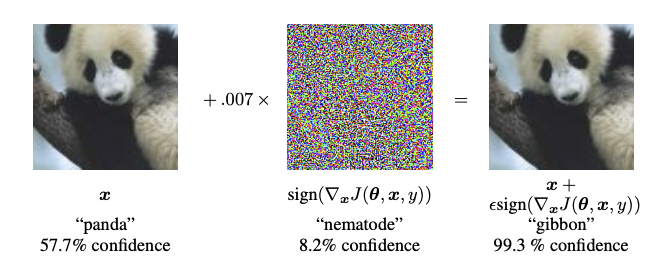
\includegraphics[width=0.8\linewidth]{Images/FGSM.png}
    \end{figure}
    \begin{center}
    \tiny{Adversarial example using FGSM, Tensorflow, 2024}
    \end{center}
    The core idea of FGSM is to choose a perturbation that locally maximizes the loss function.

    The linear approximation of the loss function with respect to $\Delta$ is given by
    \begin{equation}\label{eq:FGSM_linear_approx}
     L(X+\Delta,Y;\theta)\simeq L(X,Y;\theta)+\sum_{k,\ell}(\nabla_{X}L(X,Y;\theta))_{k\ell}\Delta_{k\ell}
    \end{equation}
    where the subscript $(\cdot)_{k\ell}$ denotes the $(k,\ell)$ component.
    The right-hand side of~\eqref{eq:FGSM_linear_approx} is maximized by choosing $\Delta_{k\ell}=\epsilon\,{\rm sign}(\nabla_{X}L(X,Y;\theta))_{k\ell}$, whose matrix form is given by
    \[
     \Delta = \epsilon\, {\rm sign}(\nabla_{X}L(X,Y;\theta)).
    \]
\end{frame}
\begin{frame}{Threat Model}
    \begin{figure}[H]
      \centering
      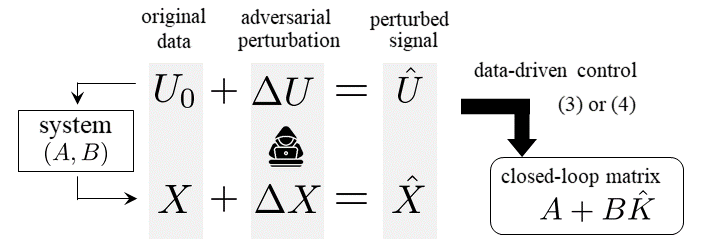
\includegraphics[width=0.6\linewidth]{scenario.png}
      \caption{\cite{10383531}, Threat model.

      The adversary is able to add a perturbation $(\Delta U, \Delta X)$ to the original input and output data $(U_0,X)$ with knowledge of the system model, the signals, and the controller design algorithm.
      The controller $\hat{K}$ is designed using the perturbed data $(\hat{U},\hat{X})$, which results in the closed-loop matrix $A+B\hat{K}$.
      }
      \label{fig:scenario}
    \end{figure}
    \begin{definition}[Transferability]
    The effectiveness of the attack without knowledge of the data
    \end{definition}
    \begin{center}
        \tiny{Adversarial attacks to direct data-driven control for destabilization, Hampei Sasahara, 2023}
    \end{center}
\end{frame}
\begin{frame}[allowframebreaks]{Directed Gradient Sign Method}
\begin{figure}[H]
  \centering
  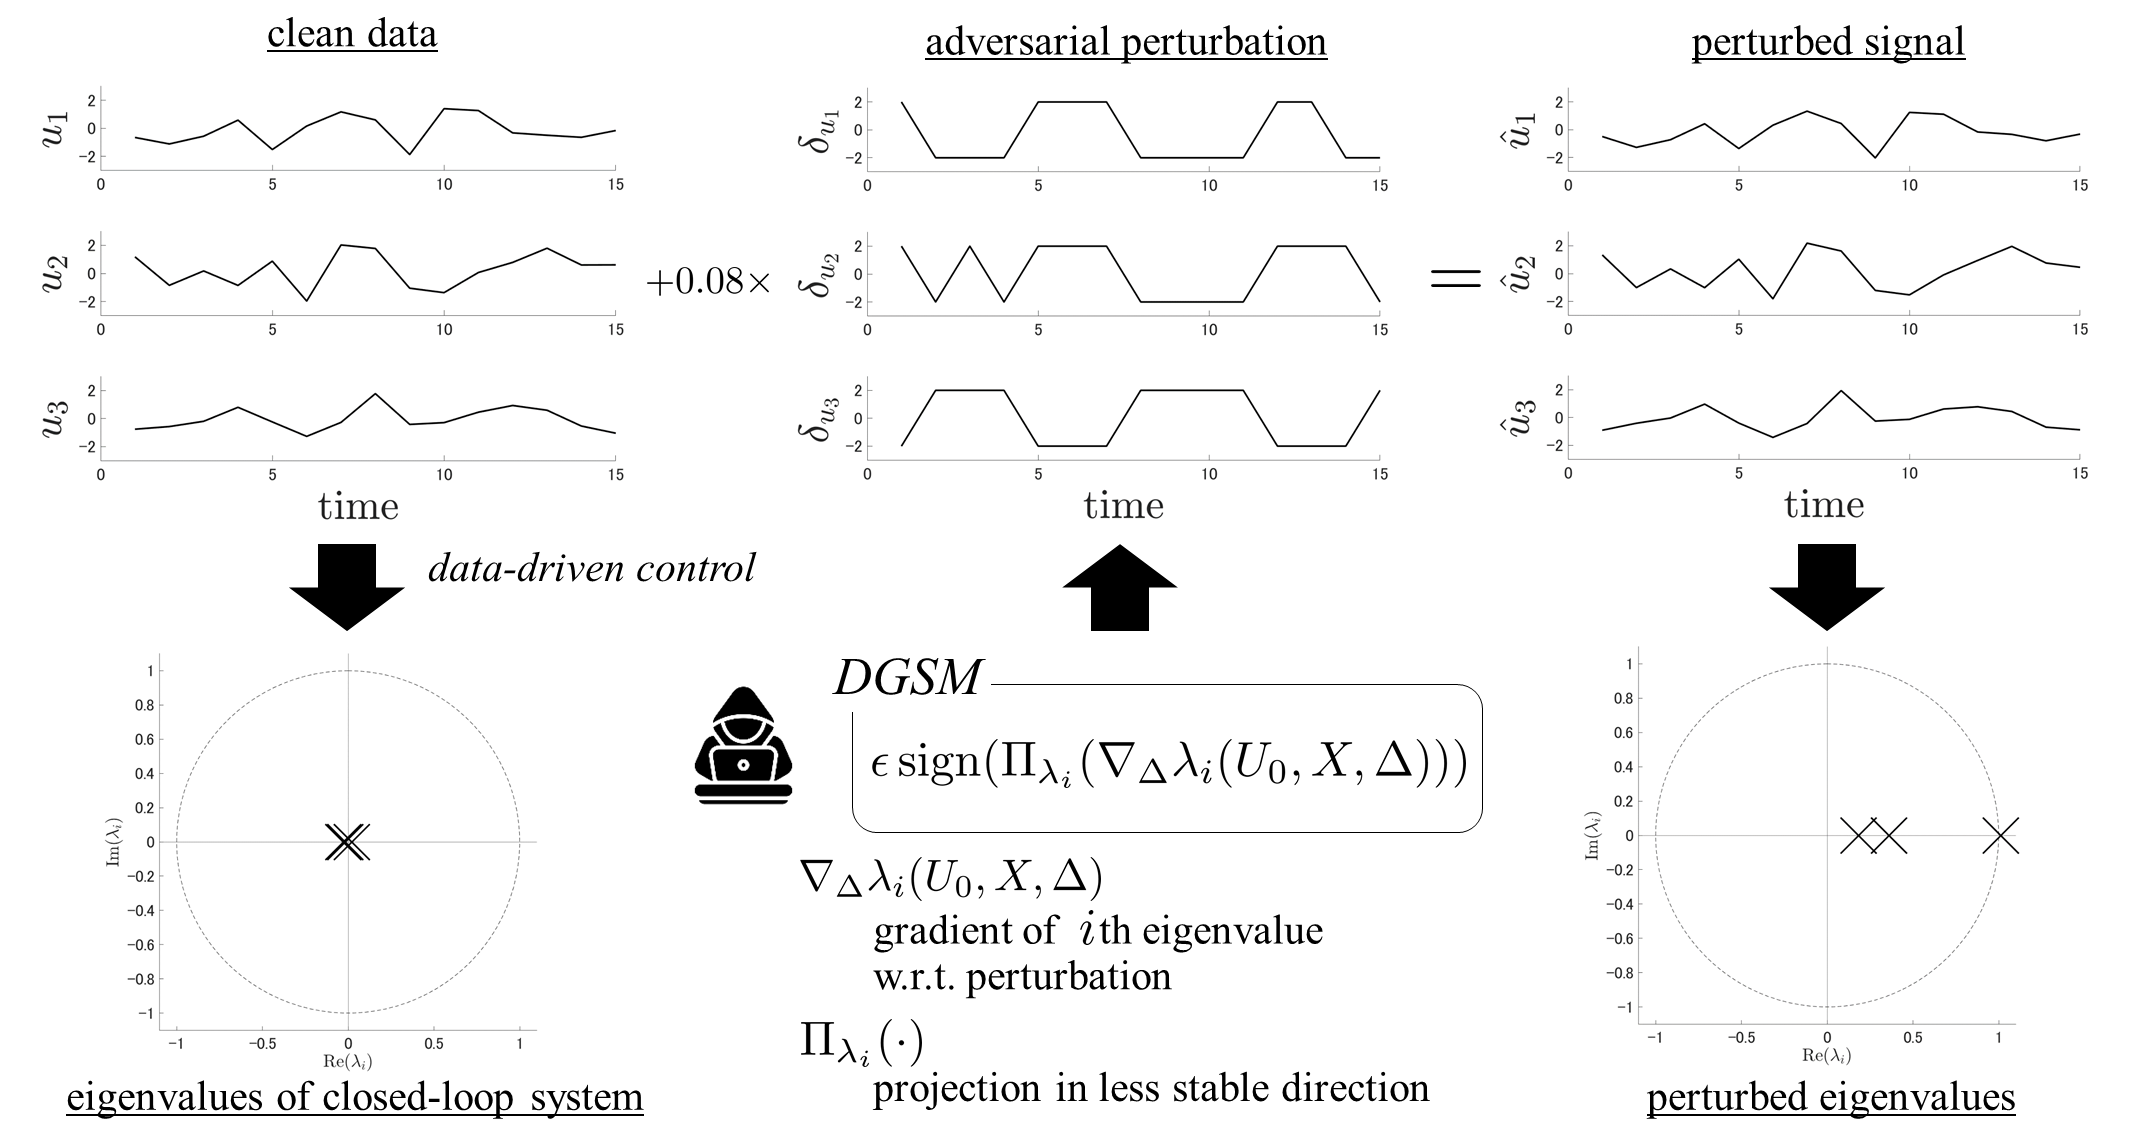
\includegraphics[width=0.7\linewidth]{Images/vulnerable_instance.png}
  \caption{\cite{10383531},
  Demonstration of DGSM applied to a discrete-time linear system with three-dimensional input.
  % The adversarial perturbation created by DGSM is added to the original signal, but the perturbed signal appears almost identical to the original one.
  % Nevertheless, the resulting closed-loop system obtained through direct data-driven control with a regularizer becomes unstable due to the adversarial attack.
  % Indeed, the eigenvalues of the closed-loop system with the clean data are $\{-0.0177, 0.0212, -0.0275\}$, while those with the perturbed data are $\{0.1824, 0.3613, 1.0120\}$.
  % %The specific parameters of this instance are provided in Sec.~\ref{subsec:vuln_ins}.
  % The specific parameters of this instance are provided in Appendix.
  % Note that the output signal is also perturbed but its illustration is omitted for clarity.
  }
  \label{fig:vuln_ins}
\end{figure}
\begin{center}
\tiny{Adversarial attacks to direct data-driven control for destabilization, Hampei Sasahara, 2023}
\end{center}
\begin{figure}[H]
% \centering
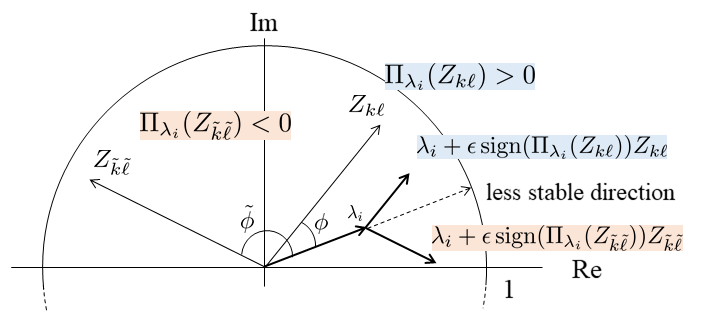
\includegraphics[width=0.6\linewidth]{Pi.png}
\caption{\cite{10383531}, Role of the function $\Pi_{\lambda_i}$ in~\eqref{eq:Pi}.
  % for scalar variables $z$ and $\tilde{z}$.
  Since $Z_{k\ell}$ faces the direction of $\lambda_i$, the angle $\phi$ between $\lambda_i$ and $Z_{k\ell}$ is less than $\pi/2$, which leads to $\Pi_{\lambda_i}(Z_{k\ell})>0$.
  On the other hand, since $\tilde{\phi}$ between $\lambda_i$ and $Z_{\tilde{k}\tilde{\ell}}$ is greater than $\pi/2$, $\pi_{\lambda_i}(Z_{\tilde{k}\tilde{\ell}})<0$.
  As a result, in both cases, the perturbed eigenvalue moves closer to the unit circle.}
\end{figure}
\begin{center}
    \tiny{Adversarial attacks to direct data-driven control for destabilization, Hampei Sasahara, 2023}
    \end{center}
\begin{figure}[H]
The core idea of DGSM is to choose a perturbation that locally shifts an eigenvalue in the less stable direction.
%the gradient of an eigenvalue moves in the less stable direction.
We temporarily fix the eigenvalue of interest, denoted by $\lambda_i(U_0,X,\Delta)$,
and denote its gradient with respect to $\Delta$ by $\nabla_{\Delta}\lambda_i(U_0,X,\Delta)$.
%We hereinafter focus on a single eigenvalue $\lambda_i$, and let $\lambda_i(U_0,X,\Delta)$ be the $i$th element of $\Lambda(U,X,\Delta)$.
%We denote the gradient of $\lambda_i(U_0,X,\Delta)$ with respect to $\Delta$ by $\nabla_{\Delta}\lambda_i(U_0,X,\Delta)$.
%The aim of the attack is to place $\lambda_i(U_0,X,\Delta)$ outside the unit circle.
%The core idea of DGSM is to choose a perturbation such that the gradient moves in the less stable direction.
The linear approximation of the eigenvalue with respect to $\Delta$ is given by
\begin{equation}\label{eq:DGSM_linear_approx}
 \lambda_i(U_0,X,\Delta)\simeq \lambda_i(U_0,X,0)+\sum_{k,\ell} \nabla_{\Delta}\lambda_i(U_0,X,\Delta)) \Delta_{k\ell}.
\end{equation}
We choose $\Delta_{k \ell}$ such that the right-hand side of~\eqref{eq:DGSM_linear_approx} moves closer to the unit circle.
Specifically, DGSM crafts the perturbation
\[
 \Delta = \epsilon\, {\rm sign}(\Pi_{\lambda_i}(\nabla_{\Delta}\lambda_i(U_0,X,\Delta)))
\]
where $\Pi_{\lambda_i}:\mathbb{C}^{(m+n)\times(2T+1)}\to \mathbb{R}^{(m+n)\times(2T+1)}$ is defined by
\begin{equation}\label{eq:Pi}
 \Pi_{\lambda_i}(Z):= \Real{\lambda_i}\Real{Z}+\Imag{\lambda_i}\Imag{Z} \qquad\text{with}\qquad Z:=\nabla_{\Delta}\lambda_i(U_0,X,\Delta).
\end{equation}
%$Z:=\nabla_{\Delta}\lambda_i(U_0,X,\Delta).$
% \centering
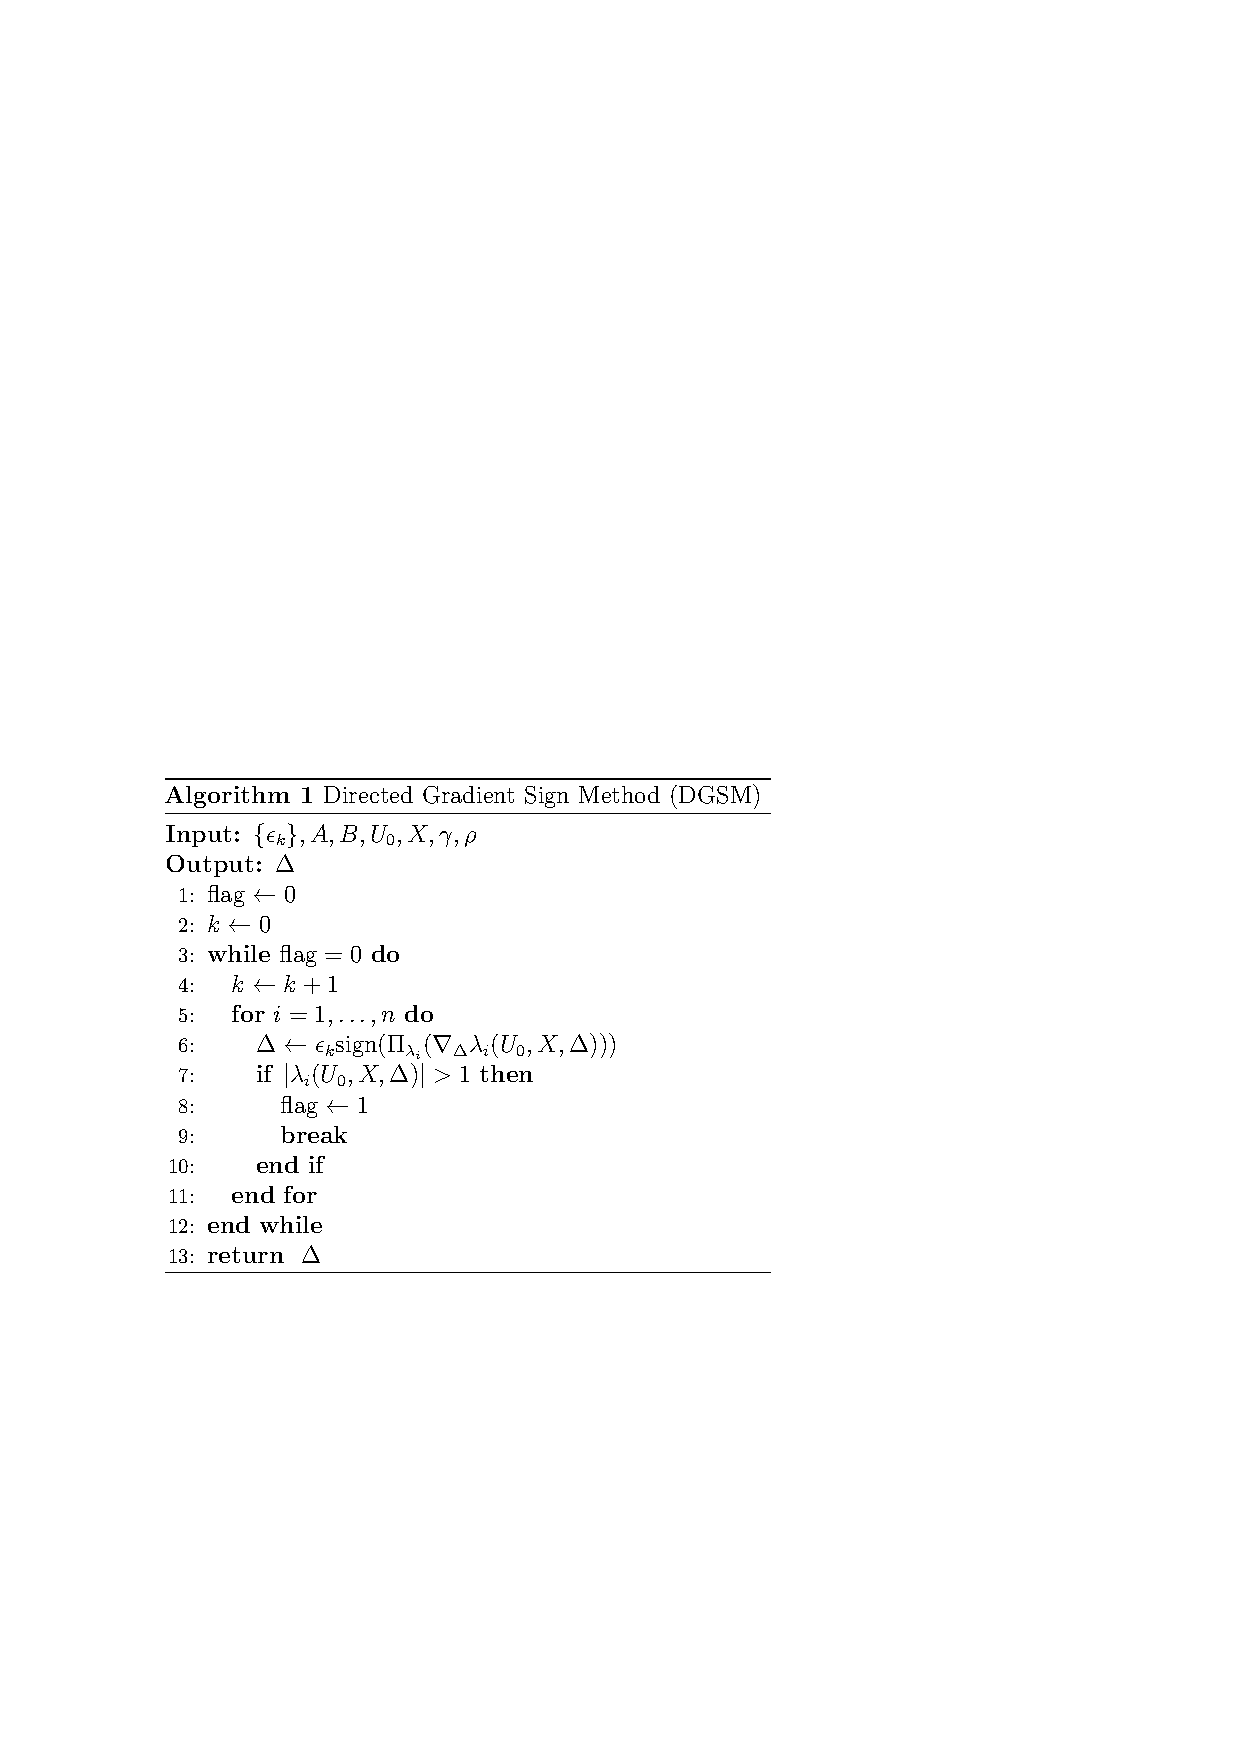
\includegraphics[width=0.4\linewidth]{DGSM.pdf}
\caption{\cite{10383531}, The Algorithm.}
\end{figure}
\begin{center}
\tiny{Adversarial attacks to direct data-driven control for destabilization, Hampei Sasahara, 2023}
\end{center}
\end{frame}
\begin{frame}{Conclusions and Future Work}
        \begin{itemize}
            \item Stabilisation algorithms are susceptible to adversarial attacks
            \item Performance of other control objectives against adversarial attacks
            \item Development of stronger attack models
            \item System simulation
        \end{itemize}
\end{frame}
\section{References}
\begin{frame}[allowframebreaks]
  \frametitle<presentation>{References}
%   \bibliographystyle{plainnat}    
\bibliographystyle{plainurl}
  % \s{*}
  {\bibliography{references}}
%   \begin{thebibliography}{10}
    
%   \beamertemplatebookbibitems
%   % Start with overview books.

%   \bibitem{Author1990}
%     A.~Author.
%     \newblock {\em Handbook of Everything}.
%     \newblock Some Press, 1990.
 
    
%   \beamertemplatearticlebibitems
%   % Followed by interesting articles. Keep the list short. 

%   \bibitem{Someone2000}
%     S.~Someone.
%     \newblock On this and that.
%     \newblock {\em Journal of This and That}, 2(1):50--100,
%     2000.
%   \end{thebibliography}
\end{frame}
\end{document}